\documentclass[format=acmsmall,screen,timestamp=false,a4paper]{acmart}
\pdfoutput=1
\newif\ifarxiv
\arxivtrue


\ifarxiv
\setkeys{acmart.cls}{nonacm}
\settopmatter{printccs=false,printacmref=false}
\else
\setkeys{acmart.cls}{draft}
\fi
\setcopyright{none}
\acmDOI{}

\acmJournal{TOMS}

\usepackage{amsmath}
\usepackage{caption}
\usepackage{subcaption}
\usepackage{pgfplots}
\usepackage{pgfplotstable}
\pgfplotscreateplotcyclelist{mycolor}{
  red,every mark/.append style={fill=red},mark=*\\
  blue,every mark/.append style={fill=blue},mark=*\\
  orange,every mark/.append style={fill=orange},mark=*\\
  red,densely dotted, every mark/.append style={fill=red},mark=square*\\
  blue,densely dotted, every mark/.append style={fill=blue},mark=square*\\
  orange,densely dotted every mark/.append style={fill=orange},mark=square*\\
}

\usepackage{listings}
\usepackage{xspace}
\usepackage{booktabs}
\usepackage{multirow}
\lstloadlanguages{python}

% Default listing language
\lstset{language=python,
  basicstyle=\footnotesize\ttfamily,
  showspaces=false,
  showtabs=false,
  frame=tb,
  numbers=left,
  xleftmargin=0em,
  xrightmargin=0em}

\DeclareMathOperator{\Div}{div}
\DeclareMathOperator{\curl}{curl}

\newcommand{\R}{\mathbb{R}}
\newcommand{\red}[1]{\textcolor{red}{#1}}
\newcommand\akg[1]{\textbf{\textcolor[rgb]{.5,0,1}{[Andrew: #1]}}}
\newcommand\josh[1]{\textbf{\textcolor[rgb]{0,.5,1}{[Josh: #1]}}}
\newcommand\justin[1]{\textbf{\textcolor[rgb]{0,1,0.5}{[Justin: #1]}}}
\newcommand\lm[1]{\textbf{\textcolor[rgb]{1,0,0.5}{[Lawrence: #1]}}}
\newcommand\rck[1]{\textbf{\textcolor[rgb]{1,0.5,0.5}{[Rob: #1]}}}
\newcommand{\calP}{\mathcal{P}}
\newcommand{\calQ}{\mathcal{Q}}
\newcommand{\calS}{\mathcal{S}}
\newcommand{\hcurl}{\ensuremath{{H}(\curl)}\xspace}
\newcommand{\hdiv}{\ensuremath{{H}(\Div)}\xspace}

\newcommand{\cancel}[1]{}

%%
%% end of the preamble, start of the body of the document source.

%%
%% The "title" command has an optional parameter,
%% allowing the author to define a "short title" to be used in page headers.
\title[Trimmed Serendipity elements in Firedrake]{Bringing Trimmed Serendipity Methods to Computational Practice in Firedrake}

%%
%% The "author" command and its associated commands are used to define
%% the authors and their affiliations.
%% Of note is the shared affiliation of the first two authors, and the
%% "authornote" and "authornotemark" commands
%% used to denote shared contribution to the research.

\author{Justin Crum}
\email{jcrum@math.arizona.edu}
\affiliation{%
  \institution{University of Arizona}
  \city{Tucson}
  \state{Arizona}
}

\author{Cyrus Cheng}
\email{cyrus.cheng15@alumni.imperial.ac.uk}
\affiliation{%
  \institution{Imperial College}
  \city{London}
  \country{United Kingdom}
}

\author{David Ham}
\affiliation{%
  \institution{Imperial College London}
  \department{Department of Mathematics}}
\email{david.ham@imperial.ac.uk}

\author{Lawrence Mitchell}
\orcid{0000-0001-8062-1453}
\affiliation{%
  \institution{Durham University}
  \department{Department of Computer Science}}
\email{lawrence.mitchell@durham.ac.uk}

\author{Robert Kirby}
\affiliation{%
  \institution{Baylor University}
  \city{Waco}
  \state{Texas}
}
\email{robert_kirby@baylor.edu}

\author{Joshua A. Levine}
\affiliation{%
  \institution{University of Arizona}
}
\email{josh@email.arizona.edu}

\author{Andrew Gillette}
\affiliation{%
  \institution{University of Arizona}
  \city{Tucson}
  \state{Arizona}}
\email{agillette@math.arizona.edu}
%%
%% By default, the full list of authors will be used in the page
%% headers. Often, this list is too long, and will overlap
%% other information printed in the page headers. This command allows
%% the author to define a more concise list
%% of authors' names for this purpose.
%\renewcommand{\shortauthors}{Trovato and Tobin, et al.}

%%
%% The abstract is a short summary of the work to be presented in the
%% article.

\begin{abstract}
       We present an implementation of the trimmed serendipity finite element family, using the open source finite element package Firedrake.  The new elements can be used seamlessly within the software suite for problems requiring $H^1$, \hcurl~or \hdiv-conforming elements on meshes of squares or cubes.  To test how well trimmed serendipity elements perform in comparison to traditional tensor products elements, we perform a sequence of numerical experiments including the primal Poisson, mixed Poisson, and Maxwell cavity eigenvalue problems.  Overall, we find that the trimmed serendipity elements converge, as expected, at the same rate as the respective tensor product elements while being able to offer significant savings in the time or memory required to solve certain problems.
\end{abstract}
  

% Use \cref and \Cref for references and everything "works out"
\usepackage[capitalise]{cleveref}

\begin{document}
  \maketitle
  
  
  \section{Introduction}
  
  In addition to the four families of finite elements present on the Periodic Table of Finite Elements \cite{arnold2014periodic}, recent research has examined a fifth family, called the \emph{trimmed serendipity finite elements}.  Similar to their tensor product and ``regular'' serendipity counterparts,  trimmed serendipity elements provide another finite element method for approximating the solution to partial differential equations on square or cubical meshes.  While potential computational advantages of these new elements have been described in previous works, they have never been realized or tested in a modern finite element package.  In particular, the serendipity and trimmed serendipity elements should attain the same rate of convergence as tensor product elements while requiring fewer degrees of freedom (DOFs) to do so.  By implementing the trimmed serendipity and tensor product elements in the same software package, we seek to make these elements available to the broader finite element community while assessing their computational advantages in a common and practical setting for the first time.
  
  %(The prior sentence will need further revisions - just taking a stab at it.  The previous sentence: To remedy this, we will present an implementation in Firedrake for $H^1$-, $H($curl$)$, and $H($div$)$ conforming trimmed serendipity elements in both $n=2,3$ dimensions for arbitrary orders $r$.)

\begin{figure}[htbp]
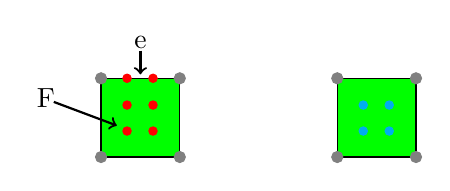
\begin{tikzpicture}
%\filldraw [gray] (0,0,0) circle (2pt);
\filldraw [green] (0,0,1) -- (1,0,1) -- (1,1,1) -- (0,1,1) -- cycle;

%\filldraw [gray] (0,1,0) circle (2pt);
%\filldraw [gray] (1,0,0) circle (2pt);
%\filldraw [gray] (1,1,0) circle (2pt);

%\draw[dotted] (0,0,0) -- (0,0,1); %x is the third component
%\draw[dotted] (0,0,0) -- (1,0,0); %y is the first component 
%\draw[dotted] (0,0,0) -- (0,1,0); %z is the second component
%\filldraw [cyan] (0,0,1) -- (1,0,1) -- (1,1,1) -- (0,1,1) -- cycle;
%\draw (0,1,0) -- (1,1,0); 
%\draw (0,1,0) -- (0,1,1);
\draw (0,1,1) -- (1,1,1);
%Josh: thickening to make really stand out.
%\draw[cyan,line width=2] (0,1,1) -- (1,1,1);
\draw (0,0,1) -- (0,1,1);
\draw (0,0,1) -- (1,0,1);
%\draw (1,0,0) -- (1,0,1);
\draw (1,0,1) -- (1,1,1);
%\draw (1,0,0) -- (1,1,0);
\draw[thick, ->] (0.5,1.35,1) -- (0.5,1.05,1);
\draw (0.5,1.45,1) node {e};
\draw[thick, ->] (-0.6,0.7,1) -- (0.2,0.4,1);
\draw (-0.7,0.75,1) node {F};
%\filldraw [red] (1,1,0.33) circle (1.5pt);
%\filldraw [red] (1,1,0.66) circle (1.5pt);
\filldraw [red] (0.33,0.66,1) circle (1.5pt);
\filldraw [red] (0.33,0.33,1) circle (1.5pt);
\filldraw [red] (0.66,0.33,1) circle (1.5pt);
\filldraw [red] (0.66,0.66,1) circle (1.5pt);
\filldraw [red] (.33,1,1) circle (1.5pt);
\filldraw [red] (.66,1,1) circle (1.5pt);


%Josh: drawing front circles on top
\filldraw [gray] (0,0,1) circle (2pt);
\filldraw [gray] (0,1,1) circle (2pt);
\filldraw [gray] (1,0,1) circle (2pt);
\filldraw [gray] (1,1,1) circle (2pt);

%\draw[thick, ->] (3,0,0) -- (3,0,1);
%\draw[thick, ->] (3,0,0) -- (3,1,0);
%\draw[thick, ->] (3,0,0) -- (4,0,0);
%\draw (3,0,1.3) node {x};
%\draw (3,1.2,0) node {z};
%\draw (4.2,0,0) node {y};

%\filldraw [gray] (0,0,0) circle (2pt);
\filldraw [green] (3,0,1) -- (4,0,1) -- (4,1,1) -- (3,1,1) -- cycle;

%\filldraw [gray] (0,1,0) circle (2pt);
%\filldraw [gray] (1,0,0) circle (2pt);
%\filldraw [gray] (1,1,0) circle (2pt);

%\draw[dotted] (0,0,0) -- (0,0,1); %x is the third component
%\draw[dotted] (0,0,0) -- (1,0,0); %y is the first component 
%\draw[dotted] (0,0,0) -- (0,1,0); %z is the second component
%\filldraw [cyan] (0,0,1) -- (1,0,1) -- (1,1,1) -- (0,1,1) -- cycle;
%\draw (0,1,0) -- (1,1,0); 
%\draw (0,1,0) -- (0,1,1);
\draw (3,1,1) -- (4,1,1);
%Josh: thickening to make really stand out.
%\draw[cyan,line width=2] (0,1,1) -- (1,1,1);
\draw (3,0,1) -- (3,1,1);
\draw (3,0,1) -- (4,0,1);
%\draw (1,0,0) -- (1,0,1);
\draw (4,0,1) -- (4,1,1);
%\draw (1,0,0) -- (1,1,0);
%\draw[thick, ->] (3.5,1.35,1) -- (3.5,1.05,1);
%\draw (3.5,1.45,1) node {e};
%\draw[thick, ->] (2.4,0.7,1) -- (3.2,0.4,1);
%\draw (2.3,0.75,1) node {F};
%\filldraw [red] (1,1,0.33) circle (1.5pt);
%\filldraw [red] (1,1,0.66) circle (1.5pt);
\filldraw [cyan] (3.33,0.66,1) circle (1.5pt);
\filldraw [cyan] (3.33,0.33,1) circle (1.5pt);
\filldraw [cyan] (3.66,0.33,1) circle (1.5pt);
\filldraw [cyan] (3.66,0.66,1) circle (1.5pt);
%\filldraw [red] (3.33,1,1) circle (1.5pt);
%\filldraw [red] (3.66,1,1) circle (1.5pt);


%Josh: drawing front circles on top
\filldraw [gray] (3,0,1) circle (2pt);
\filldraw [gray] (3,1,1) circle (2pt);
\filldraw [gray] (4,0,1) circle (2pt);
\filldraw [gray] (4,1,1) circle (2pt);


\end{tikzpicture}
\caption{The \texttt{RTCF} tensor product element \cite{raviart1977mixed} (left) used in \cref{lst:mixedPoissonCode} where we indicate DOFs on the face and one edge as an example.  The \texttt{RTCF} element is an example of a tensor product element in 2D, which depending upon the orientation of the DOFs on the edges, can be used for either \hdiv or \hcurl problems.  The right displays a similar example for the \texttt{DQ} element, which is an $L^2$-conforming tensor product element in 2D, and is necessary to form the stable pair for the mixed Poisson problem.\label{fig:RTCF}}
%The reference cube $[0,1]^3$ is shown, with coordinate axes indicated.  The edge $e$ lies in the intersection of the planes $y=1$ and $z=1$.  To ensure proper continuity, basis functions associated to $e$ must vanish on all edges of the cube \textit{except} $e$.  Examples of such functions for $e$ are described in detail in the text.  Additional examples of functions associated to the face $F$ are also given.\label{fig:RTCF}}
\end{figure}
  
In this paper, we present a complete implementation of the trimmed serendipity element family in 2D and 3D within the Firedrake finite element package \cite{rathgeber2016firedrake}, accompanied by a suite of numerical experiments demonstrating their approximation accuracy and potential benefits on benchmark partial differential equation problems.
Firedrake is a Python package for computing the solution to PDEs by using the finite element method.  By leveraging the Unified Form Language \cite{Logg:2012,alnaes2014unified}, it is able to provide a flexible and high level interface for the solution of PDEs that is reminiscent of their mathematical formulation.

%Firedrake is a Python package that uses the FEniCS problem solving language and the Unified Form Language (UFL) \cite{Logg:2012,alnaes2014unified} to provide a flexible and high level interface to the solution of PDEs close to their mathematical formulation.

An example of writing a discretized PDE and computing its approximate solution in Firedrake can be found in \cref{lst:mixedPoissonCode}. To do this, we first write the mixed Poisson equation on the domain $\Omega := [0, 1] \times [0,1]$ with boundary $\Gamma$ in the (continuous) weak formulation.  We assume homogeneous Dirichlet boundary conditions so that the integral over $\Gamma$ is $0$.  The problem statement is then:
find $\sigma \in \Sigma :=~$\hdiv and $u \in V := L^2$ such that:%\akg{Justin: Where did you get this formulation from? It seems like it should be fv not f nu in the second equation.  Also, doesn't the BC make the integral over Gamma = 0?}

\begin{equation}\label{eq:MixedPoisson}
\begin{tabular}{rllll}

$\displaystyle\int_\Omega (\sigma \cdot \tau + \nabla\cdot\tau u) \text{ d}x$ & $=~~\displaystyle \int_\Gamma \tau \cdot n u \text{ d}x$ & $\forall~ \tau\in\Sigma$, \\
$\displaystyle\int_\Omega \nabla \cdot \sigma v \text{ d}x$ & $= ~~\displaystyle -\int_\Omega fv \text{ d}x$ & $\forall~ v\in V$.
\end{tabular}
\end{equation}

 %\lm{I had a go at fixing this, but the formulation is still imprecise. What are the boundary data, what are $\Sigma$ and $V$?}
Solving the discretized version of this requires choosing a suitable pair of finite element spaces to create a stable method.  On a mesh of squares, the typical stable pair of finite elements would be \texttt{RTCF} and \texttt{DQ} for the \hdiv and $L^2$ elements, respectively.  (Later we will use the trimmed serendipity pair \texttt{SminusDiv} and \texttt{DPC} as an alternative stable pair).  We demonstrate this tensor product pairing in \cref{lst:mixedPoissonCode}, where the order of the vector and scalar elements are offset by 1 in accordance with the theory for optimal convergence rates.

%\akg{Here is a revised equation with the formatting I was describing.  Please check for correctness.  You can put it using integral notation instead of parentheses. Then after stating it you can say ``We assume Neumann boundary conditions so that the boundary integral over $\Gamma$ is 0'' or something like that. }
  
\begin{lstlisting}[float=htpb,caption={Basic Firedrake implementation of the mixed Poisson problem showcasing where to choose the elements that are used and how to create the equations in Firedrake's notation.}, label={lst:mixedPoissonCode}, numbers=left, firstnumber=1, xleftmargin=20pt,  xrightmargin=20pt]
polyDegree = 2
numberOfCells = 2**5
mesh = UnitSquareMesh(numberOfCells, numberOfCells, quadrilateral=True)
hDivSpace = FunctionSpace(mesh, "RTCF", polyDegree)
l2Space = FunctionSpace(mesh, "DQ", polyDegree - 1)
mixedSpace = hDivSpace * l2Space

sigma, u = TrialFunctions(mixedSpace)
tau, v = TestFunctions(mixedSpace)

x, y = SpatialCoordinate(mesh)
uex = sin(pi*x)*sin(pi*y)

f = -div(grad(uex))
a = (dot(sigma, tau) + div(tau)*u + div(sigma)*v)*dx
l = -f*v*dx
w = Function(mixedSpace)
solve(a == l, w)
\end{lstlisting}


  
  
An important strength of Firedrake is its modular structure for both users and developers.
For the user, swapping to trimmed serendipity elements to solve the mixed Poisson problem is now only a matter of modifying lines 4--5 in \cref{lst:mixedPoissonCode} to the appropriate identifiers, \texttt{SminusDiv} and \texttt{DPC} inside the \texttt{FunctionSpace} calls that define \texttt{HDivSpace} and \texttt{L2Space}.
%\josh{Shouldn't these be HDivSpace and L2Space?}
   %While ease of use for practitioners is one reason for choosing Firedrake as a library for implementing trimmed serendipity elements, it is not the only one.    
   For developers, implementing a new element type -- such as trimmed serendipity -- is simply a matter of defining a suitable computational basis and connecting it to the intermediate interfaces in the included libraries.  We implement the basis functions from~\cite{gillette2019computational} (that are already associated to portions of the square or cube geometry) within FIAT, and then Firedrake's form compiler generates the code for the variational forms.
   
   Having these available in Firedrake allows users to test the theoretical limits that the trimmed serendipity elements are trying to attain.  In 2D, the trimmed serendipity elements at low orders have fewer, though similar, numbers of DOFs to tensor product and serendipity elements.  However, as the degree of the elements is increased, the gap between the number of DOFs for trimmed serendipity elements and tensor product elements grows.  
   
   
\begin{figure}[htbp]
  \centering
  \begin{subfigure}[h]{0.3\textwidth}
    \begin{tikzpicture}[scale=0.5]
      \begin{semilogyaxis}[xlabel={Degree}, ylabel={DOFs},
             ylabel near ticks, ymax=1e6, ymin=1e4, xmax=6, xmin=1,
             legend pos=south east, legend style={font=\tiny} ,
             cycle list name=mycolor]
        \addplot
        table [x=Degree,y=Dofs, col sep=comma]{csvs/SerendipityDegDofsTwo.csv};
        \addlegendentry{$S^- \Lambda^0$}
        \addplot
        table [x=Degree,y=Dofs, col sep=comma]{csvs/LagrangeDegDofs.csv};
        \addlegendentry{$Q^-\Lambda^0$}
      \end{semilogyaxis}
      \end{tikzpicture}
      \caption{$H^1$-conforming elements\label{fig:2dProjectionH}}
    \end{subfigure}
    \begin{subfigure}[h]{0.3\textwidth}
      \begin{tikzpicture}[scale=0.5]
      \begin{semilogyaxis}[xlabel={Degree}, ylabel={DOFs},
             ylabel near ticks, ymax=4e6, ymin=2e4, xmax=6, xmin=1,
             legend pos=south east, legend style={font=\tiny} ,
             cycle list name=mycolor]
        \addplot
        table [x=Degree,y=Dofs, col sep=comma]{csvs/SminusCurlDegDofs.csv};
        \addlegendentry{$S^- \Lambda^1$}
        \addplot
        table [x=Degree,y=Dofs, col sep=comma]{csvs/NCEDegDofs.csv};
        \addlegendentry{$Q^-\Lambda^1$}
      \end{semilogyaxis}
      \end{tikzpicture}
      \caption{\hcurl-conforming elements\label{fig:2dProjection}}
  \end{subfigure} %\\[0.5\baselineskip]
  \begin{subfigure}[h]{0.3\textwidth}
    \begin{tikzpicture}[scale=0.5]
      \begin{semilogyaxis}[xlabel={Degree}, ylabel={DOFs},
             ylabel near ticks, ymax=4e6, ymin=2e4, xmax=6, xmin=1,
             legend pos=south east, legend style={font=\tiny} ,
             cycle list name=mycolor]
        \addplot
        table [x=Degree,y=Dofs, col sep=comma]{csvs/SminusDivDegDofs.csv};
        \addlegendentry{$S^- \Lambda^2$}
        \addplot
        table [x=Degree,y=Dofs, col sep=comma]{csvs/NCFDegDofs.csv};
        \addlegendentry{$Q^-\Lambda^2$}
      \end{semilogyaxis}
      \end{tikzpicture}
      \caption{\hdiv-conforming elements\label{fig:2dProjectionH}}
    \end{subfigure}
  \caption{We show a comparison of the DOFs required for using a trimmed serendipity element vs a tensor product element.  In each of the plots, the left-most point represents order $r=2$, and then the order increases by $1$ at each point.  The DOFs were calculated using a $[0,1]^3$ mesh that was uniformly subdivided so that each row and column of the mesh has $N=16$ elements, yielding a total mesh size of $16^3$ cubes.  The red trendlines represent the trimmed serendipity elements while the blue trendlines represent the tensor product elements.\label{fig:DegsDofs}} 
\end{figure}
   
   
   
   While the formulae for the dimensions of each space are somewhat involved, a simple count of DOFs in a standard case highlights the potential gains.
   To implement a standard mixed method for Darcy flow with quadratic order error decay in the velocity estimate, the divergence of the velocity and the pressure, on a single cube the pair of tensor product elements used have a total of 44 DOFs.
   For the same setup, the appropriate pair of regular serendipity elements have 43 DOFs, but the pair of trimmed serendipity elements have only 25 DOFs. 
   This reduces the number of DOFs by 42\% (from tensor product to trimmed serendipity), with no theoretical loss in the order of accuracy.
   
   Further, the number of DOFs shared between adjacent faces in this context is reduced by 25\% -- from 4 per face to 3 per face -- which has a dramatic impact on the global degrees of freedom for the problem.
   Such reductions increase with the approximation degree, meaning the computational savings accrued by trimmed serendipity should be most dramatic at large degree.  
   Seeing how such back-of-the-envelope calculations might bear out in a practical context requires the thorough implementation provided in this paper.
   
  Finally, we are interested in different ways to compare tensor product and trimmed serendipity elements.  The first way we discuss is a direct comparison between tensor product and trimmed serendipity elements of the same order.  This will yield a comparison where the DOFs required for trimmed serendipity are lower than the DOFs required for tensor product elements, the rates of convergence are the same, but the constant for trimmed serendipity elements is worse.  The second way we do this analysis is to focus on trimmed serendipity elements of one order higher than the tensor product elements.  This compares elements with similar numbers of DOFs, but the trimmed serendipity method has a higher rate of convergence.

   
   
   %\akg{The rest of the intro goes into a detailed example as we discussed but I don't think this is the right place for it.  This fits more naturally into Section 3 where the notation will already have been defined and it makes sense to go into some detail.  Instead, I think the intro should have 1-2 more paragraphs highlighting the expected benefits of trimmed serendipity elements (huge reduction in DoFs in 3D, for higher order) and summarizing the major contributions.  We can discuss at our next meeting.}
   %Combinations of these sets of basis functions are what will create the basis functions for the trimmed serendipity reference element.  For instance, a basis for $\calS^-_r\Lambda^1(\square_3)$, the trimmed serendipity $H($curl$)$-conforming element in 3D, can be decomposed as
   
   %\begin{equation}\label{eq:HCurlTrimmedSerendipityBasis}
   %\calS^-_r\Lambda^1(\square_3) =    \left[\bigoplus_{i=0}^{r-1} E_i %\Lambda^1\right]\oplus\left[ \bigoplus_{i=2}^{r-1}F_i \Lambda^1\right] \oplus %\left[\tilde{F}_r \Lambda^1\right]\oplus\left[ \bigoplus_{i=4}^{r-1}I_i \Lambda^1 %\right] \oplus \left[\tilde{I}_r \Lambda^1\right].
   %\end{equation}
   
  %Functions here have the basic naming scheme that any set denoted with a $V$ are functions defined on the vertices, sets denoted with $E$ or $\tilde{E}$ are functions defined on the edges, sets denoted with $F, \tilde{F}, \hat{F}$ are functions defined on the faces, and the sets denoted with an $I$ or $\tilde{I}$ are defined on the interior of the cube in 3d. 
  
  %\begin{example}\label{ex:UsingComputationalBasis}
  %To illustrate how \cref{eq:HCurlTrimmedSerendipityBasis} works, consider the case of $\calS_1^-\Lambda^1(\square_3)$.  In this scenario, $r=1$, and so we ignore the sets $F_i\Lambda^1$, $\tilde{F}_r\Lambda^1$, $I_i \Lambda^1$ and $\tilde{I}_r\Lambda^1$.  This means we only need to focus on the functions associated to the edge of the reference element.  These functions form a basis of $12$ functions that all have the form of
  
  %\begin{equation*}
  %    (y\pm 1)(z\pm 1)dx + (x\pm 1)(z\pm 1) dy + (x \pm 1)(y \pm 1)dz.
  %\end{equation*}
  
  %Notice that, give a specific edge of $\square_3$, we can identify exactly one of the 12 possible basis functions to it.  For example, if we are interested in the edge such that $y=1, z=1$, we know that $dy = dz = 0$, and thus the only nonzero basis function must be nonzero in the $dx$ component. Therefore, the $y=1, z=1$ edge is associated to the basis function $(y+1)(z+1)dx$.  This is an important aspect of the basis functions that Firedrake makes use of to ensure that basis functions are associated to the proper degree of freedom on the reference element.
  %\end{example}
  
Summarizing, the contributions of this paper are that we:
\begin{enumerate}
\item show how the Firedrake software environment can be used to implement trimmed serendipity elements and allow a user to work with these elements with only small changes to their existing code, 
\item illustrate trimmed serendipity finite elements achieving the theoretical bounds that are predicted in terms of convergence rates, and  
\item examine the costs and benefits of using trimmed serendipity elements within the confines of typical test problems for numerical analysis by comparing them to tensor product elements.
\end{enumerate}
  
  
  %In the next section, we will give more background on the trimmed serendipity elements that will explain where these basis functions come from.  This is followed by an explanation of what Firedrake is and how it makes implementing and using new finite elements easy in the third section.  Finally in section 4, we focus on various numerical experiments comparing the efficiency of using tensor product and trimmed serendipity elements.  
  
\section{Background and notation for trimmed serendipity elements}
   
    Over the last 15 years, conforming finite element methods for Hodge-Laplace type problems on simplicial and cubical meshes have been categorized using the language of Finite Element Exterior Calculus (FEEC)~\cite{AFW2006,AFW2010,ABB2012}.  Among its many advantages, FEEC gives an easy, unified way to notate different element types.  The four best known families of elements are denoted $\calP^-_r \Lambda^k$, $\calP_r \Lambda^k$, $\calQ^-_r \Lambda^k$, and $\calS_r \Lambda^k$, which are, respectively, the trimmed polynomial, polynomial, tensor product, and serendipity elements of order $r$ using $k$-forms.  The $\calP$ and $\calP^-$ spaces are defined over meshes of simplices (triangles, tetrahedra, etc) while the $\calQ^-$ and $\calS$ spaces are defined over meshes of hypercubes (squares, cubes, etc). The optional notation $(\square_n)$ specifies that the space is constructed over the $n$-dimensional cube in $\R^n$, but we will frequently omit this addition if $n$ is clear from context.
    
    The mathematical results from FEEC regarding these four families families synthesize decades of research into what constitutes a stable finite element, i.e.\ a numerical method that can be proven to converge to the correct solution of certain PDEs in certain norms at a prescribed rate, indicated by the subscript $r$.  In any dimension, the $0$-form spaces provide scalar-valued, $H^1$-conforming elements.  In 2D, $1$-forms can represent both \hcurl~and \hdiv~elements, depending on the orientation of the DOFs defined on the edges of a mesh.  In 3D, $1$-forms correspond to \hcurl~elements while $2$-forms correspond to \hdiv~elements.  Notably, the serendipity family $\calS_r\Lambda^k$ is the youngest, least implemented, and hence least understood among all these families.  In particular, the 1-form and 2-form (regular) serendipity elements in 3D were only characterized in 2014 by Arnold and Awanou~\cite{arnold2014finite}, whereas the equivalent tensor product elements were first described by N\'ed\'elec in the 1980s~\cite{N1980,N1986}.
 
 
\begin{table}[htbp]
  \centering
\begin{tabular}{rm{.14\textwidth}m{.05\textwidth}m{.14\textwidth}m{.05\textwidth}m{.14\textwidth}m{.05\textwidth}m{.14\textwidth}m{.05\textwidth}}
% $n=3$\\
 & $\qquad\calS_r^-\Lambda^0(\square_3)$ && $\qquad\calS_r^-\Lambda^1(\square_3)$  && $\qquad\calS_r^-\Lambda^2(\square_3)$  && $\qquad\calS_r^-\Lambda^3(\square_3)$ \\[2mm]
$r=1~~$ 
& {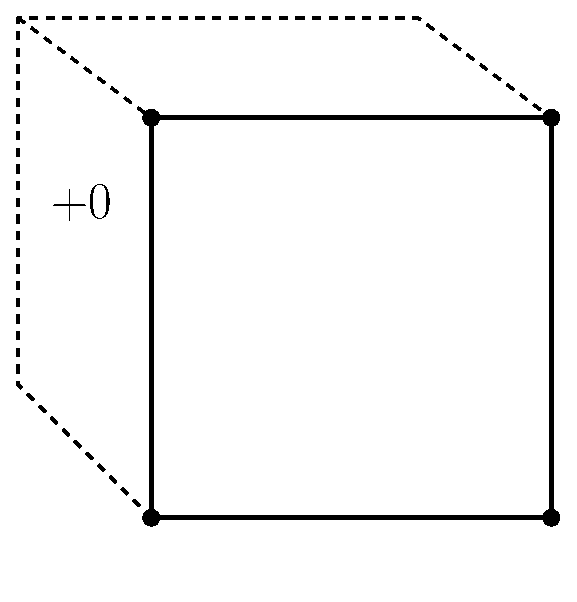
\includegraphics[width=.14\textwidth]{ts3d/Sm-103}} 
& \raisebox{8\height}{\Large 8}
& {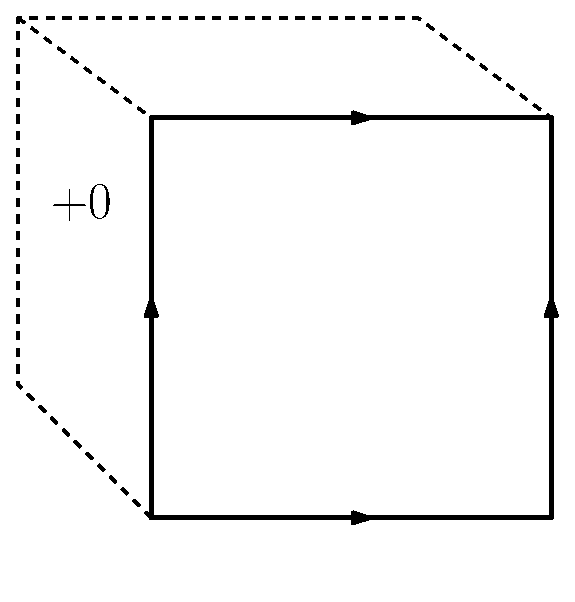
\includegraphics[width=.14\textwidth]{ts3d/Sm-113}} 
& \raisebox{8\height}{\Large 12}
& {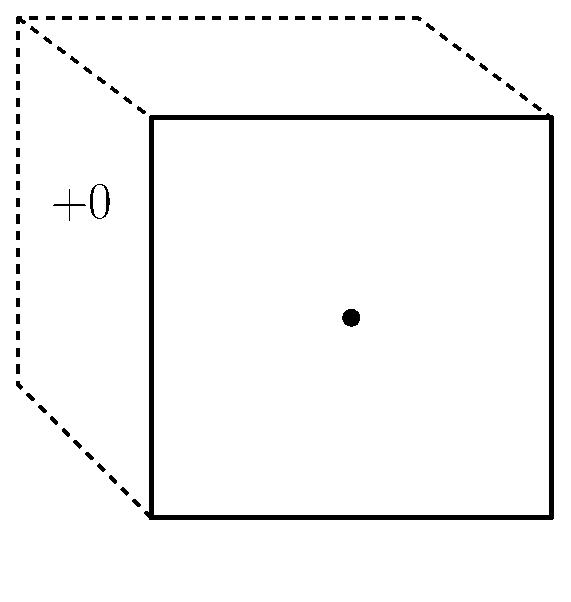
\includegraphics[width=.14\textwidth]{ts3d/Sm-123}} 
& \raisebox{8\height}{\Large 6}
& {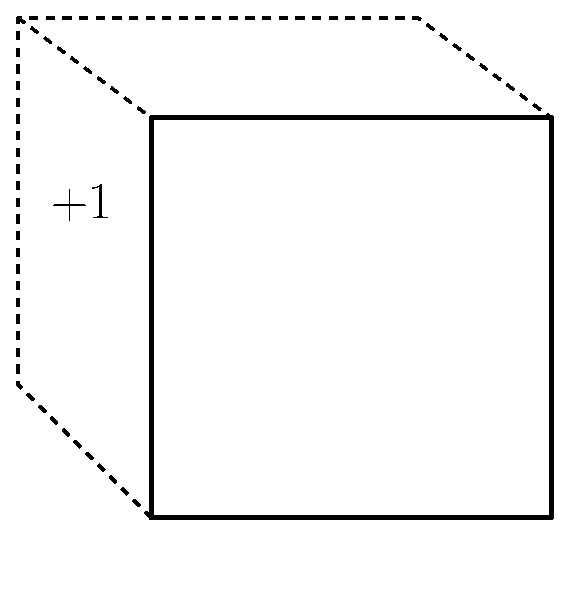
\includegraphics[width=.14\textwidth]{ts3d/Sm-133}}
& \raisebox{8\height}{\Large 1} \\
$r=2$
& {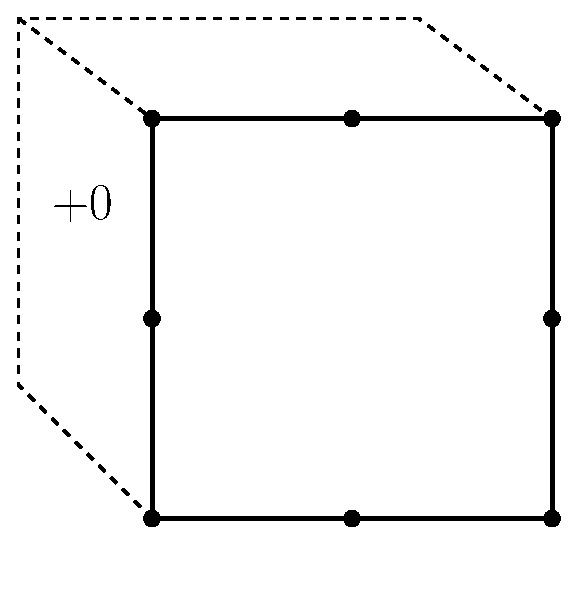
\includegraphics[width=.14\textwidth]{ts3d/Sm-203}} 
& \raisebox{8\height}{\Large 20}
& {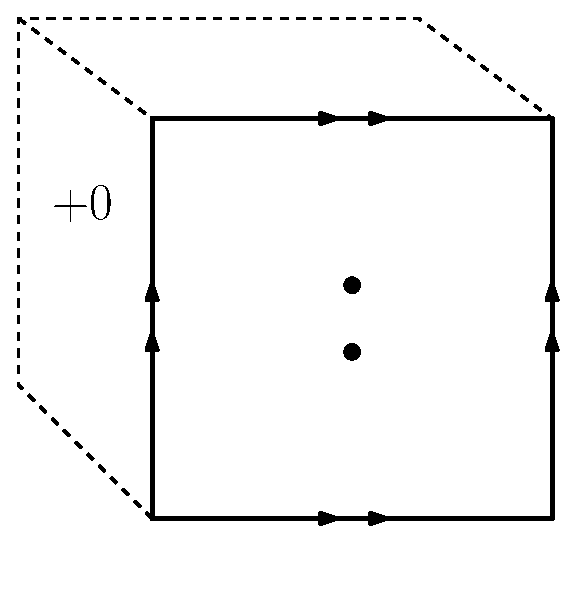
\includegraphics[width=.14\textwidth]{ts3d/Sm-213}} 
& \raisebox{8\height}{\Large 36}
& {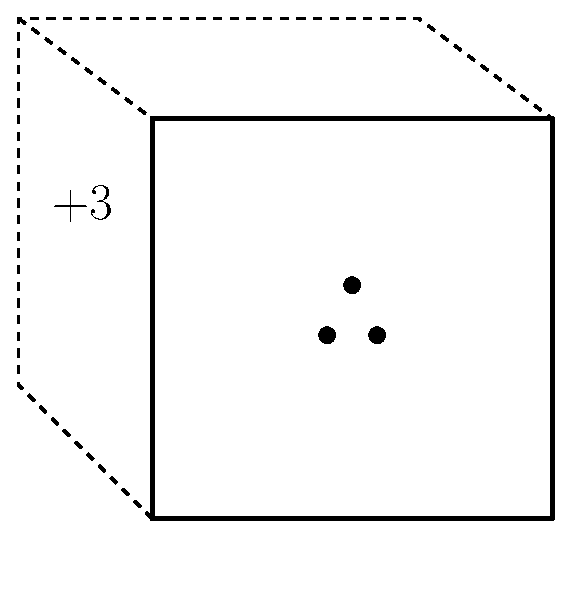
\includegraphics[width=.14\textwidth]{ts3d/Sm-223}} 
& \raisebox{8\height}{\Large 21}
& {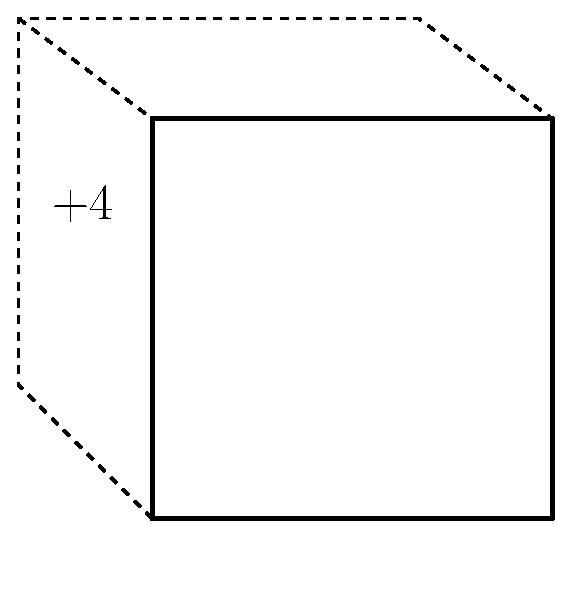
\includegraphics[width=.14\textwidth]{ts3d/Sm-233}}
& \raisebox{8\height}{\Large 4} \\
$r=3$
& {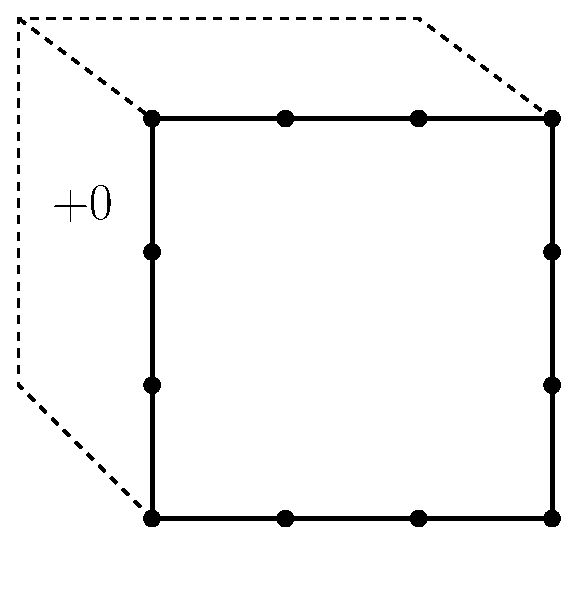
\includegraphics[width=.14\textwidth]{ts3d/Sm-303}} 
& \raisebox{8\height}{\Large 32}
& {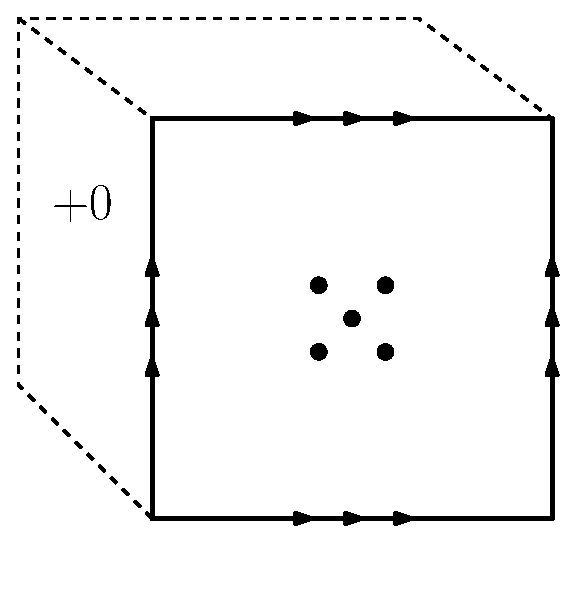
\includegraphics[width=.14\textwidth]{ts3d/Sm-313}} 
& \raisebox{8\height}{\Large 66}
& {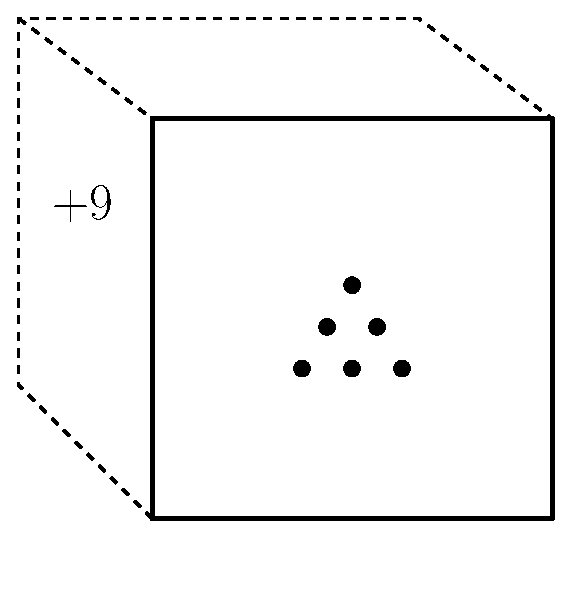
\includegraphics[width=.14\textwidth]{ts3d/Sm-323}} 
& \raisebox{8\height}{\Large 45}
& {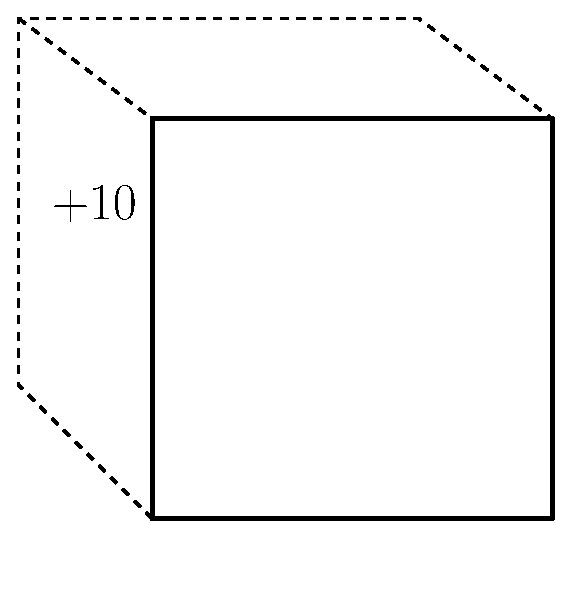
\includegraphics[width=.14\textwidth]{ts3d/Sm-333}}
& \raisebox{8\height}{\Large 10}
\end{tabular}

\caption{Trimmed serendipity elements on a reference cube in 3D, akin to the Periodic Table of the Finite Elements.  Columns show increasing form order from $k=0$ to $k=3$, corresponding to $H^1$,~\hcurl,~\hdiv, and $L^2$ conformity, respectively.  Rows show increasing order of approximation $r=1,2,3$.
On the front face of each element, dots indicate the number of DOFs associated to each vertex, edge, or face of the cubical element.  The number of DOFS associated to the interior of the cube is indicated with ``$+X$.''  The total degree of freedom count for each element is shown to its right.
}
\label{tab:tsfamily}
\end{table}


 
 
    
\subsection{Trimmed Serendipity Elements}
    The trimmed serendipity family is an even newer addition to this collection that attains a key optimality condition arising from the FEEC framework.
	In~\cite{christiansen2016constructions}, Christiansen and Gillette computed the minimal possible dimensions for an exact sequence of conforming finite element spaces on cubes that contained $\calP_r\Lambda^k$ for each $k$.
	In~\cite{gillette2019trimmed}, Gillette and Kloefkorn identified polynomial differential form spaces with these prescribed dimensions and approximation power, denoting them trimmed serendipity elements with the notation $S^-_r\Lambda^k$.  
	The trimmed serendipity spaces share the same interleaving containment structure with the serendipity spaces as the polynomial and trimmed polynomial subspaces have.  That is, for any fixed dimension $n$, any form order $0\leq k\leq n$, and any approximation order $r\geq 1$, we have both
\begin{equation*}
      \calS_r \Lambda^k \subset \calS^-_{r+1} \Lambda^k \subset \calS_{r+1} \Lambda^k
  \end{equation*}
  and   
   \begin{equation*}
      \calP_r \Lambda^k \subset \calP^-_{r+1} \Lambda^k \subset \calP_{r+1} \Lambda^k.
  \end{equation*}
	These containments express the fact that typically a finite element practitioner will get the most computational efficiency for a desired approximation order by choosing an appropriate $\calP^-$ space instead of a $\calP$ space.
	An equivalent claim is implied about serendipity and trimmed serendipity spaces, with additional comparison to the larger dimensioned tensor product spaces, $\calQ^-$, possible as well.

%	Many additional mathematical properties proved in~\cite{gillette2019trimmed} solidify the analogue between the $\calP_r^-\Lambda^k$ and $\calS_r^-\Lambda^k$ families.

    
    
%Solving partial differential equations on cubical meshes has been a topic of many different finite element studies. In 3D, this includes the $H($curl$)$ and $H($div$)$ Nedelec elements. However, this ignores the other two families of finite element differential forms for square and cubical meshes, the serendipity and trimmed serendipity elements.
  
%  In \cite{arnold2011serendipity}, Arnold and Awanou described the shape functions for serendipity elements $\calS_r$ in $n$ dimensions as the space of polynomials with superlinear degree in at most $n$ variables, denoted as $deg_2 p$, such that $deg_2 p \leq r$. This gave serendipity elements a concrete definition in $n$ dimensions. Moreover, they showed that serendipity elements defined in such a way can be assigned a set of unisolvent DOFs and that there is a nice way to give a geometric decomposition of the serendipity elements.
  

% Following this, Gillette and Kloefkorn then introduced the trimmed serendipity elements $S^-_r$ in \cite{gillette2019trimmed}.  The trimmed serendipity elements are the answer to the question ``Does there exist a minimal compatible finite element system on cubes containing $P_r \Lambda^k$?'', and contain the expected amount of interior DOFs as described by Christiansen and Gillette in \cite{christiansen2016constructions}.  
  

	As a step toward testing such ideas, Gillette, Kloefkorn and Sanders gave a systematic way to build the computational basis for each of these elements for dimensions $n = 2, 3$, $k=0, 1, 2, 3$-forms, and arbitrary order $r \geq 1$~\cite{gillette2019computational}.
  %\josh{referring back to the abstract/intro where we say ``complete'', it is my understanding our implementation supports $n=2,3$ and $k=0, \ldots, n-1$.  Do we implement $k = n$ or am I missing something?}
	These ``computational bases'' are well-suited for implementation since each basis function is associated to a unique portion a mesh element - i.e.\ a specific vertex, edge, face (for cubes) or element interior.
	The required geometric localization of DOFs is visualized for low orders in 3D in \cref{tab:tsfamily}, arranged equivalently to the Periodic Table of the Finite Elements.
	We note that neither the particular bases defined in~\cite{gillette2019computational} nor any other general implementation of trimmed serendipity elements has been attempted prior to this paper.

	
	
  %Using these basis functions, we implemented the trimmed serendipity elements in 2 and 3 dimensions inside of Firedrake, a python package for solving partial differential equations using finite element methods. 
  %  The trimmed serendipity elements in both 2D and 3D can be defined in terms of the $k$-forms used to represent them, or the type of space they conform to.
  
  
  \subsubsection{Scalar Trimmed Serendipity Elements}
  The scalar-valued trimmed serendipity elements that are represented by $0$-forms are used as the shape functions for an $H^1$-conforming finite element space.  These are denoted by $\calS_r^-\Lambda^0$ and are identical to the scalar-valued serendipity elements from the Periodic Table of Finite Elements, i.e.\ $\calS_r^-\Lambda^0(\square_n) = \calS_r\Lambda^0(\square_n)$ for any $n$.  Arnold and Awanou provided a simple description of the functions in $\mathcal{S}_r\Lambda^0$ as the span of all monomials of ``superlinear degree'' less than or equal to $r$~\cite{arnold2011serendipity}. 
  
  Likewise, the scalar-valued trimmed serendipity elements that are represented by $n$-forms create $L^2$-conforming finite element spaces.  These are denoted by $\calS_r^-\Lambda^n(\square_n)$, and here we have the equality $\calS_r^-\Lambda^n(\square_n) = \calS_{r+1}\Lambda^n(\square_n)$.  In terms of the Periodic Table of Finite Elements, these are the \textbf{dPc}$_r$ spaces.  The shape functions for these spaces are simply the space of order $r$ polynomials.  Since no inter-element continuity is needed for $L^2$-conformity, we have the additional equivalence $\calS_r^-\Lambda^n(\square_n) = \calP_{r+1}\Lambda^n(\square_n)$.
  
  \subsubsection{Vector-valued Trimmed Serendipity Elements}
  

	The trimmed serendipity elements are truly distinct from regular serendipity spaces for $k$ values $0<k<n$.  Here, we will only consider dimensions $n=2$ and $n=3$, where the $k$-form spaces can be identified as vector-valued finite elements.  	
	In 2D, the vector-valued spaces $\calS_r^-\Lambda^1(\square_2)$ bear close relation to the Arbogast Correa elements~\cite{arbogast2016two}, as explained in~\cite[Prop 2.2]{gillette2019trimmed}.
	In 3D, the vector valued spaces $\calS_r^-\Lambda^1(\square_3)$ and $\calS_r^-\Lambda^2(\square_3)$ were also characterized by Cockburn and Fu~\cite{CF2016}, as explained in~\cite[Prop 2.3]{gillette2019trimmed}.

	
	A major reason that the vector trimmed serendipity elements have only recently been considered in the mathematical literature is that their DOF per element count is complicated.
	As evidenced by Table~\ref{tab:tsfamily}, \textit{certain} DOFs grow in predictable patterns with $r$.
	For instance, elements in the 1-form family, $\calS_r^-\Lambda^1(\square_3)$, have exactly $r$ DOFs per edge of the cube (corresponding to ``order $r$'' approximation on edges) and elements in the 2-form family, $\calS_r^-\Lambda^2(\square_3)$, have ${\displaystyle {r+1}\choose 2}$ DOFs per face (corresponding to ``order $r$'' approximation on faces).
	However, the 2-form family has the more obscure quantity of $(r^3 - 2r^2 + 3r)/2$ DOFs associated to the interior of an element (for $r>1$).
	This growth pattern is recognized as sequence A064808 by the On-line Encyclopedia of Integer Sequences~\cite{OEIS} and is in agreement with the general formulae presented in~\cite{gillette2019trimmed}, but a natural geometric interpretation remains elusive.
	Equally unexpected patterns are evident in the growth of DOFs on faces and interiors of the $\calS_r^-\Lambda^1(\square_3)$ family.
	As we will discuss in the next section, Firedrake makes the creation and incorporation of such unusual DOF growth patterns simple for the developer, and thus opens these elements to numerical testing for the first time.
	
%	
%	\akg{Talk about Arbogast Correa paper~\cite{arbogast2016two}}
%
%\akg{Still editing from here}
%	
%%At $k=0$ and $k=n$, the trimmed serendipity spaces coincide with regular serendipity spaces, but for intermediate values of $k$ and $r>1$, the containments are strict and hence the dimensions 
%  
%  	First we look at the case $k=n-1$, i.e.\ the \hdiv-conforming element families $\calS_r^-\Lambda^1(\square_2)$ and $\calS_r^-\Lambda^2(\square_3)$. 
%	
%
%
%  The vector trimmed serendipity elements can be split into two groups: 1-forms and $(n-1)$-forms.  
%  
%  The first group normally discussed are the $2$-forms in 3D and $1$-forms in 2D, .  Both are \hdiv-conforming finite elements.  Unfortunately, the vector trimmed serendipity elements do not have a ``nice'' definition for their shape functions.  Instead, we have the definition that in general, 
%  \begin{equation*}
%      \calS_r^-\Lambda^k = \calS_{r-1}\Lambda^k + \kappa \calS_{r-1}\Lambda^{k+1}
%  \end{equation*}
%  where $\kappa$ is the Kozsul differential operator, and $k=2$ in 3D, $k=1$ in 2D.  This is a more difficult definition to work with, which emphasizes the importance of having the computational bases, such as the one shown in \cref{ex:UsingComputationalBasis}.  
%  
%  In 3D, the $1$-forms that are used to represent an \hcurl-conforming finite element space also are defined using the shape forms as described above, using $k=1$ instead of $k=2$.  In 2D, the \hcurl-conforming finite element space is simply a rotation of the \hdiv-space.  
  
 % For each of these different types of elements, we present experiments in section 4 that detail how the trimmed serendipity elements compare to the corresponding tensor product elements.  The scalar $H^1$-conforming elements are used in the primal Poisson problem, while the scalar $L^2$-conforming elements are used in the mixed Poisson problem.  For the vector elements, the \hdiv-conforming elements are used in the mixed Poisson problem while the \hcurl-conforming elements are tasked with solving the Maxwell cavity eigenvalue problem.
  
  
  \section{Building capacity for serendipity element types in Firedrake}
  \label{sec:buildcap}

  Firedrake uses the FIAT \cite{kirby2004algorithm,kirby2012fiat} to provide finite element basis functions on reference elements. 
  To implement a new element in FIAT, we must provide both rules to tabulate basis functions and their derivatives at reference element points and a data structure that assigns basis functions to particular reference element facets.
  Said element is then made available in Firedrake by providing a symbolic name (in UFL \cite{alnaes2014unified}) and a translation from symbolic name to concrete implementation in the form compiler TSFC \cite{homolya2018tsfc}. We follow the construction of \cite{gillette2019computational} which provides explicit formulae for the basis functions for each of the trimmed serendipity elements and directly implement tabulation of the basis functions rather than using a Ciarlet definition and providing a dual basis from which FIAT constructs the primal basis. To provide tabulations of derivatives, we implement the basis functions symbolically with SymPy \cite{sympy2017} and compute derivatives symbolically. %\lm{Andrew/Justin: is this actually true? Is this the implementation route? Is there something deeper than typing out the equations in \cite{gillette2019computational}?}\akg{Need to revise this paragraph after getting clarification about FIAT from Rob.}  \rck{Actually, Justin is right.  Cyrus (and Justin, following him) are bypassing CiarletElements and just providing tabulation via sympy formulae.}
  
  
We use the decompositions from~\cite{gillette2019computational} to group the basis functions according the geometric portions of a reference mesh element (vertices, edges, faces, or cell interiors).  For instance, a basis for $\calS^-_r\Lambda^1(\square_3)$ -- the trimmed serendipity $H($curl$)$-conforming element in 3D -- can be decomposed as
   \begin{equation}\label{eq:HCurlTrimmedSerendipityBasis}
   \calS^-_r\Lambda^1(\square_3) =   \underbrace{\left[\bigoplus_{i=0}^{r-1} E_i \Lambda^1\right]}_{\text{edge functions}}\oplus\underbrace{\left[ \bigoplus_{i=2}^{r-1}F_i \Lambda^1\right] \oplus \left[\tilde{F}_r \Lambda^1\right]}_{\text{face functions}}\oplus\underbrace{\left[ \bigoplus_{i=4}^{r-1}I_i \Lambda^1 \right] \oplus \left[\tilde{I}_r \Lambda^1\right]}_{\text{interior functions}}.
   \end{equation}
  Subsets in these decompositions denoted with an $E$, $F$, or $I$ are defined on edges, faces, and interior, respectively, of the cubical cell in 3D.
  %\begin{example}\label{ex:UsingComputationalBasis}
  %To illustrate how \cref{eq:HCurlTrimmedSerendipityBasis} is implemented, consider the components of $\calS_1^-\Lambda^1(\square_3)$.  In this scenario, $r=1$, and so we ignore the sets $F_i\Lambda^1$, $\tilde{F}_r\Lambda^1$, $I_i \Lambda^1$ and $\tilde{I}_r\Lambda^1$ (to see the exact formulation for each of these sets, see Gillette \cite{gillette2019computational}).  This means we only need to focus on the functions associated to the edge of the reference element.  These functions create a basis of $12$ functions that all have the form 
  %\begin{equation*}
  %    (y\pm 1)(z\pm 1)dx + (x\pm 1)(z\pm 1) dy + (x \pm 1)(y \pm 1)dz.
  %\end{equation*}
  
  %Notice that, given a specific edge of $\square_3$, we can identify exactly one of the 12 possible basis functions to it.  For example, if we are interested in the edge such that $y=1, z=1$, we know that $dy = dz = 0$, and thus the only nonzero basis function must be nonzero in the $dx$ component. Therefore, the $y=1, z=1$ edge is associated to the basis function $(y+1)(z+1)dx$.  This is an important aspect of the basis functions that Firedrake makes use of to ensure that basis functions are associated to the proper degree of freedom on the reference element.
  
  %The next step to taking the analytic basis function from paper to code is to translate from a differential form to a vector.  We consider $dx$ as our first component of the vector, $dy$ as our second, and $dz$ as the third.  Therefore, we  think of $(y+1)(z+1)dx$ as being a vector $\big((y+1)(z+1), 0, 0\big)$.  Finally, we take the vector we've created and push that into a FIAT context \lm{I don't think I know what this means} where it is able to represent the degree of freedom on the $y=1, z=1$ edge.
  %\josh{Is this example really illustrating equation 1?  It seems like most everything is ignored because of the fact $r=1$.  More generally, it's unclear that someone reading this knows what to implement from the brief description here...could we elaborate more?  For me, it's missing the mark.}
  %\lm{I agree with this comment. I think we need to figure out what the core ``computational mathematics'' contribution is.}
  %\end{example}
 
To see how this plays out in the Firedrake implementation, consider the \hcurl~elements for trimmed serendipity at order $r=2$ in $n=3$ dimensions, indicating the space $S_2^- \Lambda^1$ in 3D. According to \cref{eq:HCurlTrimmedSerendipityBasis}, the basis functions can be decomposed as
\begin{equation}\label{eq:HcurlRtwo}
   \calS^-_2\Lambda^1(\square_3) =    \left[\bigoplus_{i=0}^{1} E_i \Lambda^1\right] \oplus \left[\tilde{F}_2 \Lambda^1\right]\oplus \left[\tilde{I}_2 \Lambda^1\right].
   \end{equation}
The space $\tilde{I}_r \Lambda^1$ is defined to be empty for $r<4$, so there are only two sets of functions to include in this case: one set associated to edges of the reference element (the $E_i\Lambda^1$ sum) and one set for the faces of the reference element (the $\tilde{F}_2\Lambda^1$ functions).

We then implement these in Firedrake as follows.  The first step is to determine the number of DOFs we will need on the reference element where we will define the basis functions.  To do this, we count the DOFs for each mesh entity on the reference element (vertex, edge, face, and interior).  For example, $\mathcal{S}_2^- \Lambda^1(\square_3)$ should have no DOFs at the vertices (these only come into play for the $H^1$-conforming elements), two DOFs on each edge, two DOFs on each face, and no DOFs on the interior.  This agrees with \cref{eq:HcurlRtwo}, where $E_i\Lambda^1$ supplies one DOF to each edge for each $i=0, 1$, and then $\tilde{F}_2\Lambda^1$ supplies two DOFs to each face.  An illustration of this can be seen in the second column, second row of \cref{tab:tsfamily}.

With the number of DOFs assigned to each mesh entity in the reference element, we can then define the basis functions.  The order of definition is important so that basis functions are matched to the proper mesh entity.  Note that \cref{eq:HcurlRtwo} doesn't explicitly give a way to order the basis functions.  Instead, we need to use the properties of the basis functions to determine the correct ordering.   This is best illustrated by an example. Two of the ``edge'' basis functions that are contained in the sum of the $E_i\Lambda^1$ sets are $(y+1)(z+1)dx$ and $x(y+1)(z+1)dx$.  Notice that these functions have no $dy$ or $dz$ portions.  Therefore, these function vanish on any edge \textit{not} parallel to the $x$ axis.  Further, the polynomial coefficients of these forms indicate that they also vanish on the planes $y=-1$ and $z=-1$.  Thus, the only edge of the cube on which these functions do \textit{not} vanish is the edge contained in the line $\{y=1\}\cap\{z=1\}$.  This edge is shown in blue and labeled with an ``e'' in \cref{fig:ReferenceCube}.
%we associate these functions to an edge such that the $y$ and $z$ values are constant, ensuring 0 coefficients in $dy$ and $dz$ terms.  If we choose either $y = -1$ or $z = -1$, then the two basis functions we're working with both become zero.  Therefore, we  require that both $y = 1$ and $z = 1$ for the edge that we are working with (seen as the blue edge labeled with an "e" that has 2 red dots on \cref{fig:ReferenceCube}).


\begin{figure}[htbp]
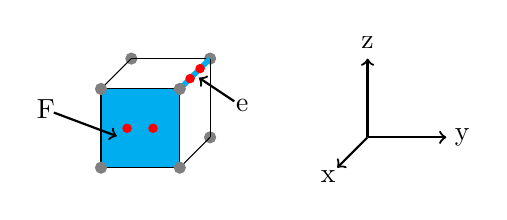
\begin{tikzpicture}
%\filldraw [gray] (0,0,0) circle (2pt);
\filldraw [cyan] (0,0,1) -- (1,0,1) -- (1,1,1) -- (0,1,1) -- cycle;

\filldraw [gray] (0,1,0) circle (2pt);
\filldraw [gray] (1,0,0) circle (2pt);
\filldraw [gray] (1,1,0) circle (2pt);

%\draw[dotted] (0,0,0) -- (0,0,1); %x is the third component
%\draw[dotted] (0,0,0) -- (1,0,0); %y is the first component 
%\draw[dotted] (0,0,0) -- (0,1,0); %z is the second component
%\filldraw [cyan] (0,0,1) -- (1,0,1) -- (1,1,1) -- (0,1,1) -- cycle;
\draw (0,1,0) -- (1,1,0); 
\draw (0,1,0) -- (0,1,1);
\draw (0,1,1) -- (1,1,1);
%Josh: thickening to make really stand out.
\draw[cyan,line width=2] (1,1,0) -- (1,1,1);
\draw (0,0,1) -- (0,1,1);
\draw (0,0,1) -- (1,0,1);
\draw (1,0,0) -- (1,0,1);
\draw (1,0,1) -- (1,1,1);
\draw (1,0,0) -- (1,1,0);
\draw[thick, ->] (1.5,0.65,0.5) -- (1.05,0.95,0.5);
\draw (1.6,0.6,0.5) node {e};
\draw[thick, ->] (-0.6,0.7,1) -- (0.2,0.4,1);
\draw (-0.7,0.75,1) node {F};
\filldraw [red] (1,1,0.33) circle (1.5pt);
\filldraw [red] (1,1,0.66) circle (1.5pt);
\filldraw [red] (0.66,0.5,1) circle (1.5pt);
\filldraw [red] (0.33,0.5,1) circle (1.5pt);

%Josh: drawing front circles on top
\filldraw [gray] (0,0,1) circle (2pt);
\filldraw [gray] (0,1,1) circle (2pt);
\filldraw [gray] (1,0,1) circle (2pt);
\filldraw [gray] (1,1,1) circle (2pt);

\draw[thick, ->] (3,0,0) -- (3,0,1);
\draw[thick, ->] (3,0,0) -- (3,1,0);
\draw[thick, ->] (3,0,0) -- (4,0,0);
\draw (3,0,1.3) node {x};
\draw (3,1.2,0) node {z};
\draw (4.2,0,0) node {y};


\end{tikzpicture}
\caption{The reference cube $[0,1]^3$ is shown, with coordinate axes indicated.  The edge $e$ lies in the intersection of the planes $y=1$ and $z=1$.  To ensure proper continuity, basis functions associated to $e$ must vanish on all edges of the cube \textit{except} $e$.  Examples of such functions for $e$ are described in detail in the text.  Additional examples of functions associated to the face $F$ are also given.\label{fig:ReferenceCube}}
\end{figure}

This process is what determines the ordering for the basis functions.  If, in the first step described above where we are assigning DOFs to mesh entities, we assign the first two DOFs to be on the edge of the reference element where $y = 1$ and $z = 1$, then we must define the basis functions $(y+1)(z+1)dx$ and $x(y+1)(z+1)dx$ as our first two basis functions.

%In FIAT, $k$-forms are represeted as $k$-tuples.  For example, the 1-forms $(y+1)(z+1)dx$ and $x(y+1)(z+1)dx$ are stored as $((y+1)(z+1), 0, 0)$ $(x(y+1)(z+1),0,0)$.  In this form, we then translate the values $(y+1)$, $(z+1)$ and $x$ in different ways.  The overall conversion to FIAT notation ends with 
While the formulas above are taken from Gillette's \cite{gillette2019computational} work, these monomials have poor conditioning at higher orders. Therefore, we use Legendre functions obtained symbolically from SymPy via the \texttt{leg} function and write the differential forms in vector notation.  For our examples of $(y+1)(z+1)dx$ and $x(y+1)(z+1)dx$, we get
\texttt{tuple([(leg(j,x\_mid)*dz[1]*dy[1],0,0)])}
, where \texttt{leg(j, x\_mid)} is used for the $1$ or $x$ coefficient, and the \texttt{dy[1]} and \texttt{dz[1]} are used for the values of $(y+1)$ and $(z+1)$, respectively.  After repeating this process for each of the edges and associated basis functions, we then also do a similar process for the face functions in the set $\tilde{F}_2 \Lambda^1$.  

This process changes only slightly if we instead had considered the the $2$-forms $\mathcal{S}^-_2 \Lambda^2(\square_3)$.  In this scenario, we would have the basis functions given by the equation

\begin{equation*}
\calS^-_2\Lambda^2(\square_3) =    \left[\bigoplus_{i=0}^{1} F_i \Lambda^2\right] \oplus \left[\tilde{I}_2 \Lambda^2\right].
\end{equation*}

\noindent In this case, one of the basis functions is $y^jz^k(x+1)dydz$.  The $dydz$ represents a $2$-form, which vanishes on any face \textit{not} parallel to the $yz$ plane.  This leaves only the faces contained in the planes $x=1$ or $x=-1$ as possibilities for association. 
As in the 1-form example above, the polynomial coefficient of the form indicates that this function will vanish on an additional mesh entity, namely, the face contained in the plane $x=-1$, in this case.
Hence, we associate this function with the face contained in $x=1$ (labeled with an ``F'' in \cref{fig:ReferenceCube}).  The rest of the process for defining the $2$-form basis functions is similar to the process for the $1$-form basis functions.
%Similar to the previous example, this time we end up with edge DOFs being defined by the functions 
%\begin{equation*}
%    x^i(y\pm 1)(z\pm 1)dx + y^i(x\pm 1)(z\pm 1) dy + z^i(x \pm 1)(y \pm 1)dz
%\end{equation*}
%and we choose their association to edges in the same fashion as before.  Then, we also have to add in the basis functions in $\tilde{F}_2\Lambda^1$.  The general form for these functions becomes a little more complicated, but one example of them would be $(z+1)(y^2-1)dx$.  Then substituting in $i=0, 1$ into the first set of equations will yield $24$ basis functions, 2 per each edge, while the collective $\tilde{F}_2\Lambda^1$ set gives 2 more functions per face.  Finally, we take the two sets of basis functions and combine them together into a single list of basis functions for the trimmed serendipity space $\mathcal{S}_2\Lambda^1(\square_3)$.   \lm{It feels like this paragraph just recapitulates the example, is there a reason why we do it twice?}

%\justin{Here we can put something like:  "To see the exact syntax for the FIAT classes defining the trimmed serendipity elements, see here."  and link the Zenodo github integration.}  This process allows us to define the FIAT element that Firedrake is going to use when we request \texttt{SminusCurl} function spaces.  After we have the element defined, FIAT does the numerical evaluation of the element and is wrapped into the FInAT element.  FInAT takes the numerical basis function tables and wraps them into an abstract syntax for table look-up.   \lm{I am not quite sure the point this paragraph is trying to make.}


\begin{table}[htbp]
  \centering
\begin{tabular}{llll}
  \toprule
   FEEC & UFL name (2D) & UFL name (3D) \\
  \midrule
  $\mathcal{Q}^-_r \Lambda^0$ & \texttt{Lagrange} & \texttt{Lagrange}  \\
   $\mathcal{Q}^-_r \Lambda^1$ & \texttt{RTCE} or \texttt{RTCF} & \texttt{NCE} \\
   $\mathcal{Q}^-_r \Lambda^2$ & \texttt{DQ} & \texttt{NCF}  \\
  $\mathcal{Q}^-_r \Lambda^3$ & \texttt{-} & \texttt{DQ}\\
  \midrule
  $\mathcal{S}^-_r \Lambda^0 $ & \texttt{S} & \texttt{S}  \\
  $\mathcal{S}^-_r \Lambda^1$ & \texttt{SminusCurl} or \texttt{SminusDiv} & \texttt{SminusCurl}  \\
  $\mathcal{S}^-_r \Lambda^2$ & \texttt{DPC} & \texttt{SminusDiv}\\
  $\mathcal{S}^-_r \Lambda^3$ & \texttt{-} & \texttt{DPC}\\
  \bottomrule
\end{tabular}
\caption{A translation between FEEC and Firedrake usage names for tensor product and trimmed serendipity elements.  In 2D, the $0$-forms are $H^1$ conforming spaces, the $1$-forms are \hcurl and \hdiv conforming spaces (dependent upon oreintation of the DOFs), and the $2$-forms are $L^2$ conforming spaces.  For 3D, the $0$-forms are $H^1$ conforming spaces, the $1$-forms are \hcurl conforming spaces, $2$-forms are \hdiv conforming spaces, and $3$-forms are $L^2$ conforming spaces. \label{tab:FiredrakeNames}}
%\lm{I had a go making this table nicer. The ``Element name'' column is kind of bad though, because the $\Lambda^2$ space is not an \hdiv space in 2D. Perhaps just drop that column entirely?}\label{tab:FiredrakeNames}}
\end{table}

The newly supported elements, mapping FEEC spaces onto names in UFL are shown in \cref{tab:FiredrakeNames}. Modifying the code from \cref{lst:mixedPoissonCode} to utilise trimmed serendipity spaces rather than tensor product spaces is then simply a case of replacing the element names in the \texttt{FunctionSpace} definitions with appropriate trimmed space names. Concretely, the new \texttt{FunctionSpace} definitions are shown in \cref{lst:pde_using_trimmed_serendipity}, the rest of the code remains unchanged.
\begin{lstlisting}[float=htbp,caption={Setting up Firedrake to use the trimmed serendipity elements in a mixed Poisson problem in 3D.}, label={lst:pde_using_trimmed_serendipity}, numbers=left, firstnumber=3, xleftmargin=20pt,  xrightmargin=20pt]
...
hDivSpace = FunctionSpace(mesh, "SminusDiv", polyDegree)
l2Space = FunctionSpace(mesh, "DPC", polyDegree - 1)
...
\end{lstlisting}
 
% \lm{I removed this paragraph of which files we edited, since I don't think it is enlightening. I put something in the intro to this section.}
 %  \josh{I think it would be appropriate to include a small table at this point, that both shows what the function spaces are called as in Firedrake vs. the mathematics expression (e.g. SminusCurl, SminusDiv, etc.) AND shows which function spaces they are designed to work with (e.g. DPC).  This will hopefully give more insight on how to use our implementation}


  \section{Experiments}
    
The following experiments show the benefits and costs of using trimmed serendipity elements in comparison to traditional tensor product elements.  We first present a basic projection example as a means of confirming approximation properties of our elements.  Next, we present results on a primal Poisson problem (to test $H^1$ elements), a mixed Poisson problem (to test \hdiv and $L^2$ elements), and a cavity resonator problem (to test \hcurl elements).  Since the \hcurl and \hdiv elements are only a rotation of the DOFs on the edges of elements in 2D, we do not give an experiment using \hcurl elements in 2D. 

The experiments were performed on a single cluster compute node with 2x AMD EPYC 7642 48-core (Rome) processors (2.4GHz) and 512GB of memory running CentOS 7.  For memory intensive runs where the order and mesh require more DOFs, the experiments were performed on a high memory node with 3TB of memory but an otherwise identical setup.  Each job was run by submitting a SLURM script that requested one node in isolation to ensure no other jobs were running at the same time.  We utilized on-node parallelism by requesting a full node and executing the jobs with \texttt{mpirun} set to use 24 processes, with a few exceptions for smaller cases that will be pointed out later.  Timing data was collected after first performing a dry run of the code to warm the cache and then taking the minimum time over three subsequent runs.  

%\josh{Somewhere in this section lead in we need to describe our experimental setup, which should include (1) hardware specifications and (2) software specifications (versions of firedrake, etc.)}

%\josh{On the hardware side, we can say something like ``all experiments were executed on a single cluster compute node with 2x AMD EPYC 7642 48-core (Rome) processor, running at 2.4GHz and with 512GB of memory.''  We should also indicate that are largest runs used a node with 3TB of memory}

%\josh{We should also state a little on how we executed these jobs, e.g. reveal some of the specs of the SLURM script we used, such as ``we utilized on node parallelism by executing these jobs with mpirun set up with KK processes''.}

%\josh{We'll also want to clarify if we had the node entirely cleared of other running jobs (I believe we did!) and thus we can modify the above to state it is free of other jobs.}

%\josh{We'll also want to mention things like ``cache warming'', ''how many runs you averaged together'', etc.  Anything we think a reasonably capable reader needs to know to reproduce our experimental results}

%\josh{Is the newpage intentional?}

%\newpage


\subsection{Projection}
  
%<<<<<<< wence/edits
We solve an $L^2$ projection problem to give a baseline accuracy test for the elements. Given either the unit square or unit cube as our domain of integration on definite integrals, we compute the projection of $f$ into the function space $V$ by using a discretization of the problem: find $u\in V$ such that
\begin{equation*}
  \int_\Omega u \cdot v \text{ d}x = \int_\Omega g \cdot v \text{ d}x, \text{ where } g = \nabla f
\end{equation*}
for all $v \in V$.  For our experiments, we choose $V$ to be \hcurl spaces for the proper dimension (see \cref{tab:FiredrakeNames}) and $f = \text{sin}(\pi x)\text{sin}(\pi y)$ or $f=\text{sin}(\pi x)\text{sin}(\pi y)\text{sin}(\pi z)$ for two or three dimensions respectively.
%\akg{What is $V$?  Since the projection figure only talks about~\hcurl, I think $V=$\hcurl.  Also what is the $f$ that you use?}
Recall that the trimmed serendipity elements are denoted with $\mathcal{S}_r^-$ and the tensor product elements with $\mathcal{Q}^-_r$.  In Firedrake, the trimmed serendipity elements use the label \texttt{SminusCurl} or \texttt{SminusDiv} for 1-forms in 2D, depending upon the orientation of the edge DOFs, and in 3D, they represent the 1- and 2-forms respectively.  The tensor product elements use the labels \texttt{RTCE} (or \texttt{RTCF}) and  \texttt{NCE} for 1-forms in 2D and 3D, while the 2-forms in 3D are  \texttt{NCF}.  To solve the projection problem, we use a Galerkin $L^2$ projection into $V$



%\josh{What domain, how did you discretize it?  Mesh resolution, etc.?  May always want to clarify how we ``count'' things, e.g. compute error and count DOFs (perhaps the latter is obvious though...it would be to me once i knew the mesh)}  
%=======
%  \begin{equation*}
%      \int u v  \text{ d}x = \int f v \text{ d}x \text{ for all v } \in V
%  \end{equation*}

% \noindent where $V$ is a test function space.   Recall that the trimmed serendipity elements are denoted with $\calS_r^-$ and the tensor product elements with $\calQ^-_r$, and in Firedrake, these have a variety of names.  The trimmed serendipity elements, in both 2D and 3D, fall under the labels {\fontfamily{qcr}\selectfont SminusCurl} and {\fontfamily{qcr}\selectfont SminusDiv} for 1- and 2-forms respectively.  The tensor product elements use the labels {\fontfamily{qcr}\selectfont RTCE} (or {\fontfamily{qcr}\selectfont RTCF}) and  {\fontfamily{qcr}\selectfont NCE} for 1-forms in 2D and 3D, while the 2-forms in 3D are  {\fontfamily{qcr}\selectfont NCF}. %\josh{What domain, how did you discretize it?  Mesh resolution, etc.?  May always want to clarify how we ``count'' things, e.g. compute error and count DOFs (perhaps the latter is obvious though...it would be to me once i knew the mesh)}  
%>>>>>>> master

%\josh{We also probably want to state precisely the mapping from the legend in this diagram (e.g. $S^-_k$ and $Q^-_k$ to their names in specific Firedrake function spaces (perhaps though, this is obvious?}

\begin{figure}[htbp]
  \centering
  \begin{subfigure}[h]{0.48\textwidth}
    \begin{tikzpicture}[scale=0.75]
      \begin{loglogaxis}[xlabel={h}, ylabel={Error},
             ylabel near ticks, ymax=1e-1, ymin=2e-11, xmax=0.3, xmin=0.5e-2,
             legend pos=south east, legend style={font=\tiny} ,
             cycle list name=mycolor]
        \addplot
        table [x=h,y=Error, col sep=comma]{csvs/ProjectionSminus2dO2.csv};
        \addlegendentry{$S^-_2$}
        \addplot 
        table [x=h,y=Error, col sep=comma]{csvs/ProjectionSminus2dO3.csv};
        \addlegendentry{$S^-_3$ }
        \addplot
        table [x=h,y=Error, col sep=comma]{csvs/ProjectionSminus2dO4.csv};
        \addlegendentry{$S^-_4$}
        \addplot
        table [x=h,y=Error, col sep=comma]{csvs/ProjectionRTCE2dO2.csv};
        \addlegendentry{$Q^-_2$}
        \addplot
        table [x=h,y=Error, col sep=comma]{csvs/ProjectionRTCE2dO3.csv};
        \addlegendentry{$Q^-_3$}
        \addplot[densely dotted, orange, mark=square*]
        table [x=h,y=Error, col sep=comma]{csvs/ProjectionRTCE2dO4.csv};
        \addlegendentry{$Q^-_4$}
      \end{loglogaxis}
      \end{tikzpicture}
      \caption{2D edge length vs error\label{fig:2dProjectionH}}
    \end{subfigure}
    \begin{subfigure}[h]{0.48\textwidth}
      \begin{tikzpicture}[scale=0.75]
      \begin{loglogaxis}[xlabel={DOFs}, ylabel={Error},
             ylabel near ticks, ymax=1e-1, ymin=2e-11, xmax=3e6, xmin=0.5e2,
             legend pos=south west, legend style={font=\tiny} ,
             cycle list name=mycolor]
        \addplot
        table [x=Dofs,y=Error, col sep=comma]{csvs/ProjectionSminus2dO2.csv};
        \addlegendentry{$S^-_2$}
        \addplot
        table [x=Dofs,y=Error, col sep=comma]{csvs/ProjectionSminus2dO3.csv};
        \addlegendentry{$S^-_3$ }
        \addplot
        table [x=Dofs,y=Error, col sep=comma]{csvs/ProjectionSminus2dO4.csv};
        \addlegendentry{$S^-_4$}
        \addplot
        table [x=Dofs,y=Error, col sep=comma]{csvs/ProjectionRTCE2dO2.csv};
        \addlegendentry{$Q^-_2$}
        \addplot
        table [x=Dofs,y=Error, col sep=comma]{csvs/ProjectionRTCE2dO3.csv};
        \addlegendentry{$Q^-_3$}
        \addplot[densely dotted, orange, mark=square*]
        table [x=Dofs,y=Error, col sep=comma]{csvs/ProjectionRTCE2dO4.csv};
        \addlegendentry{$Q^-_4$}
      \end{loglogaxis}
      \end{tikzpicture}
      \caption{2D DOFs vs error\label{fig:2dProjection}}
  \end{subfigure} \\[0.5\baselineskip]
  \begin{subfigure}[h]{0.48\textwidth}
    \begin{tikzpicture}[scale=0.75]
      \begin{loglogaxis}[xlabel={h}, ylabel={Error},
             ylabel near ticks, ymax=1e-1, ymin=2e-10, xmax=0.2, xmin=0.5e-2,
             legend pos=south east, legend style={font=\tiny} ,
             cycle list name=mycolor]
        \addplot
        table [x=h,y=Error, col sep=comma]{csvs/ProjectionSminus3dO2.csv};
        \addlegendentry{$S^-_2$}
        \addplot
        table [x=h,y=Error, col sep=comma]{csvs/ProjectionSminus3dO3.csv};
        \addlegendentry{$S^-_3$ }
        \addplot
        table [x=h,y=Error, col sep=comma]{csvs/ProjectionSminus3dO4.csv};
        \addlegendentry{$S^-_4$}
        \addplot
        table [x=h,y=Error, col sep=comma]{csvs/ProjectionNCE3dO2.csv};
        \addlegendentry{$Q^-_2$}
        \addplot
        table [x=h,y=Error, col sep=comma]{csvs/ProjectionNCE3dO3.csv};
        \addlegendentry{$Q^-_3$}
        \addplot[densely dotted, orange, mark=square*]
        table [x=h,y=Error, col sep=comma]{csvs/ProjectionNCE3dO4.csv};
        \addlegendentry{$Q^-_4$}
      \end{loglogaxis}
      \end{tikzpicture}
    \caption{3D edge length vs error\label{fig:3dProjectionH}}
  \end{subfigure}
  \begin{subfigure}[h]{0.48\textwidth}
  \begin{tikzpicture}[scale=0.75]
      \begin{loglogaxis}[xlabel={DOFs}, ylabel={Error},
             ylabel near ticks, ymax=3e-2, ymin=0.5e-9, xmax=4e8, xmin=0.25e4,
             legend pos=south west, legend style={font=\tiny} ,
             cycle list name=mycolor]
        \addplot
        table [x=Dofs,y=Error, col sep=comma]{csvs/ProjectionSminus3dO2.csv};
        \addlegendentry{$S^-_2$}
        \addplot
        table [x=Dofs,y=Error, col sep=comma]{csvs/ProjectionSminus3dO3.csv};
        \addlegendentry{$S^-_3$ }
        \addplot
        table [x=Dofs,y=Error, col sep=comma]{csvs/ProjectionSminus3dO4.csv};
        \addlegendentry{$S^-_4$}
        \addplot
        table [x=Dofs,y=Error, col sep=comma]{csvs/ProjectionNCE3dO2.csv};
        \addlegendentry{$Q^-_2$}
        \addplot
        table [x=Dofs,y=Error, col sep=comma]{csvs/ProjectionNCE3dO3.csv};
        \addlegendentry{$Q^-_3$}
        \addplot[densely dotted, orange, mark=square*]
        table [x=Dofs,y=Error, col sep=comma]{csvs/ProjectionNCE3dO4.csv};
        \addlegendentry{$Q^-_4$}
      \end{loglogaxis}
      \end{tikzpicture}
    \caption{3D DOFs vs error\label{fig:3dProjectionDofs}}
  \end{subfigure}
  \caption{Results of solving an $L^2$ projection problem using trimmed serendipity and tensor product \hcurl elements in both 2D (top row) and 3D (bottom row).  Experiments were ran for $k$-forms for $k=0,1,2,3$ in 2D and 3D, however only the $1$-forms in 3D are displayed here.  In every case, the trimmed serendipity element trendline has the same slope as its tensor product counterpart, as expected by the theory.  In most cases, the tensor product elements perform better by these metrics, in the sense that their trendlines lie below the trimmed serendipity trendlines.  The notable exception is the quadratic case, $r=2$, where trimmed serendipity perform slightly better in terms of DOFs, in both 2D and 3D.\label{Projections}} 
\end{figure}

The goal of the projection problem is to establish that the elements attain the mathematically expected rates of convergence as mesh size decreases.  For this, we create a mesh on $[0,1]^n$ of uniformly sized squares or cubes, where we refine the mesh from $N=4$ squares (or cubes) in each row and column to $N=128$ squares in each row and column (or $N=64$ cubes).  This results in a mesh with $N^2$ or $N^3$ squares or cubes respectively.  For the folllowing results, we will use $h = \frac{1}{N}$ since the mesh elements are all uniformly sized. 
We employ both trimmed serendipity elements and tensor product elements on each mesh and record the $L^2$ error in each case.  In \cref{Projections}, we report the $L^2$ error in terms of the classical measure of maximum edge length ($h$) as well as total number of degrees of freedoms (DOFs).

The expectation is that $\mathcal{S}^-_r$ and $\mathcal{Q}^-_r$ converge at the same rate with respect to $h$, which is confirmed in the plots by parallel trendlines.  These parallel trendlines can be seen in each of the projection plots.  For $r=2$, we see the trendline for $\mathcal{S}^-_r$ below the trendline for $\mathcal{Q}^-_r$, indicating that that the trimmed serendipity elements achieve a better accuracy for the amount of DOFs required than the tensor product elements.  

For the $r=2$ case, the trimmed serendipity elements achieve a better accuracy while requiring less DOFs.  Therefore in this low order case, trimmed serendipity elements would be beneficial to use.  In the case of $r=3,4$ the trendlines for $\mathcal{S}^-_r$ are above the trendlines for $\mathcal{Q}^-_r$.  However, considering the elements $\mathcal{Q}^-_3$ and $\mathcal{S}^-_4$, we see that $\mathcal{Q}^-_3$ requires approximately $1.71 \times 10^8$ DOFs and $\mathcal{S}^-_4$ at the same mesh refinement requires $0.95 \times 10^8$ DOFs.  While $\mathcal{Q}^-_3$ attains an error of $8.96 \times 10^{-8}$, the $\mathcal{S}^-_4$ elements attain an error of $2.1 \times 10^{-9}$.  
%\akg{This needs to be explained more - where is the extra order of magnitude accuracy?  Be specific.  I also agree with Josh's (commented out) comment that we need to highlight the positive - at the very practical case of $r=2$, there is a specific benefit.  What is the impact of this to a user?  Spell it out!}.

%\josh{this paragraph is making too coarse/negative of a conclusion, isn't it?  Why are we not talking about how the lines swap as $r$ increases?}

%\newpage
 



\subsection{The Poisson Problem}
In this section we discuss results for both the primal Poisson problem and the mixed Poisson problem.  We solve the primal Poisson problem described below on a unit square domain $\Omega$ for $u \in U$:
\begin{align*}
    -\Delta u &= f \\
    \displaystyle u\vert_{\partial \Omega} &= 0
%<<<<<<< wence/edits
\end{align*}
where $f(x,y) = 2\pi^2\text{sin}(\pi x)\text{sin}(\pi y) $, yielding the solution $u(x,y) = \text{sin}(\pi x)\text{sin}(\pi y)$. In 3D, we can extend this to $f(x,y,z) = 3\pi^2\text{sin}(\pi x)\text{sin}(\pi y)\text{sin}(\pi z)$ with the solution $u(x,y,z) = \text{sin}(\pi x)\text{sin}(\pi y)\text{sin}(\pi z)$ on the unit cube.  The primal Poisson equation is as follows: find $u \in V:= H^1(\Omega)$ such that:
\begin{equation*}
    \int_\Omega \nabla u \cdot \nabla v \text{ d}x = \int_\Omega f v \text{ d}x,\qquad \text{for all $v \in V$}.
\end{equation*}
Accordingly, the primal Poisson problem employs $H^1$ elements, using \texttt{S} for $\mathcal{S}^-_r \Lambda^0$ and \texttt{Lagrange} for $\mathcal{Q}^-_r \Lambda^0$. 


The mixed Poisson problem introduces an intermediate variable, $\sigma$, which is solved for simultaneously.
Formally, this is: find $\sigma\in$~\hdiv and $u\in L^2$ such that:
\begin{align}
     \sigma - \nabla u &= 0 \notag \\
     \nabla \cdot \sigma &= -f \notag \\
     u\vert_{\partial \Omega} &= 0 \notag
\end{align}
In a similar fashion as for the primal Poisson problem, we can create the weak formulation of the mixed Poisson problem that we saw in \cref{eq:MixedPoisson}.  %This is: find $\sigma \in \Sigma:=$~\hdiv and $u \in V:=L^2$ such that:
%<<<<<<< wence/edits

%\begin{equation*}
%\begin{tabular}{rllll}
%$\displaystyle\int_\Omega (\sigma \cdot \tau + \nabla\cdot\tau u) \text{ d}x$ & %$\displaystyle=~~ \int_\Gamma \tau \cdot n u \text{ d}x$ & $\forall~ \tau\in\Sigma$, \\
%$\displaystyle\int_\Omega \nabla \cdot \sigma v \text{ d}x$ & $\displaystyle= ~~-\int_\Omega fv %\text{ d}x$ & $\forall~ v\in V$.
%\end{tabular}
%\end{equation*}
These equations are discretized and solved using a suitable \textit{pair} of finite elements -- one of \hdiv type and one of $L^2$ type.  We use $(\calQ_r^-\Lambda^{n-1},\calQ_r^-\Lambda^n)$ and $(\calS_r^-\Lambda^{n-1},\calS_r^-\Lambda^n)$ for dimensions $n=2$ and $n=3$.  Note that the mathematical notation here calls for $\mathcal{Q}^-_r \Lambda^{n-1}$ to be paired with $\mathcal{Q}^-_r \Lambda^n$, but the code notation will require setting the degree of the $L^2$ element one below the degree of the \hdiv element, and similar with the trimmed serendipity elements.
For both the primal Poisson and mixed Poisson problems, we solve the system using MUMPS with a sparse direct LU factorization.
The exact set of solver parameters used for the mixed Poisson problem are shown in \cref{lst:solver_parameters}.

\begin{lstlisting}[float=htbp,caption={An example of some solver parameters that we can use for the mixed Poisson problem.  The options presented here solve the algebraic system with a simplified Newton method where the Jacobian is held constant at the first iterate.  Therefore it is factored at the beginning and triangular solves are applied to it at each subsequent iteration.  This has the effect of performing iterative refinement \cite{wilkinson1994rounding}, \cite{moler1967iterative} and yields an increased accuracy for higher order discretizations on finer meshes.}, label={lst:solver_parameters}, numbers=left, firstnumber=1, xleftmargin=20pt,  xrightmargin=20pt]
...
params = {"snes_type": "newtonls",
                  "snes_linesearch_type": "basic",
                  "snes_monitor": None,
                  "snes_converged_reason": None,
                  "mat_type": "aij",
                  "snes_max_it": 10,
                  "snes_lag_jacobian": -2,
                  "snes_lag_preconditioner": -2,
                  "ksp_type": "preonly",
                  "ksp_converged_reason": None,
                  "ksp_monitor_true_residual": None,
                  "pc_type": "lu",
                  "snes_rtol": 1e-12,
                  "snes_atol": 1e-20,
                  "pc_factor_mat_solver_type": "mumps",
                  "mat_mumps_icntl_14": "200",
                  "mat_mumps_icntl_11": "2"}
...
\end{lstlisting}

%=======

%\begin{equation*}
%    \int_\Omega \sigma \cdot \tau + \nabla \cdot \tau u + \nabla \cdot \sigma v \text{ d}x = - \int_\Omega fv \text{ d}x
%\end{equation*}
%>>>>>>> master

%\lm{Can we state all these variational problems more precisely/in more standard ``Find $u\ in V$ such that ... for all $v \in V$?'' What do you think?}

%\josh{Do we want all of these equations numbered?  Earlier in the paper we left out many of them}

\begin{figure}[htbp]
  \centering
  \begin{subfigure}[h]{0.48\textwidth}
      \begin{tikzpicture}[scale=0.75]
      \begin{loglogaxis}[xlabel={DOFs}, ylabel={Error},
             ylabel near ticks, ymax=1e-4, ymin=1e-16, xmax=2e6, xmin=2e3,
             legend pos=south west, legend style={font=\tiny} ,
             cycle list name=mycolor]
        %\addplot+[only marks, orange] table [x=Dofs,y=Time,col sep=comma]{PrimalPoissonSerendipity3dO4.csv};
        \addplot
        table [x=Dofs,y=Error, col sep=comma]{csvs/PrimalPoissonSerendipity2dO2.csv};
        \addlegendentry{$S^-_2$}
        \addplot
        table [x=Dofs,y=Error, col sep=comma]{csvs/PrimalPoissonSerendipity2dO3.csv};
        \addlegendentry{$S^-_3$ }
        \addplot
        table [x=Dofs,y=Error, col sep=comma]{csvs/PrimalPoissonSerendipity2dO4.csv};
        \addlegendentry{$S^-_4$}
        \addplot
        table [x=Dofs,y=Error, col sep=comma]{csvs/PrimalPoissonLagrange2dO2.csv};
        \addlegendentry{$Q^-_2$}
        \addplot
        table [x=Dofs,y=Error, col sep=comma]{csvs/PrimalPoissonLagrange2dO3.csv};
        \addlegendentry{$Q^-_3$}
        \addplot[densely dotted, orange, mark=square*]
        table [x=Dofs,y=Error, col sep=comma]{csvs/PrimalPoissonLagrange2dO4.csv};
        \addlegendentry{$Q^-_4$}
      \end{loglogaxis}
      \end{tikzpicture}
      \caption{2D primal Poisson convergence analysis. \label{fig:2dPrimalDofs}}
  \end{subfigure}
  \begin{subfigure}[h]{0.48\textwidth}
    \begin{tikzpicture}[scale=0.75]
      \begin{loglogaxis}[xlabel={DOFs}, ylabel={Error},
             ylabel near ticks, ymax=1e-1, ymin=1e-11, xmax=2e6, xmin=3e2,
             legend pos=south west, legend style={font=\tiny} ,
             cycle list name=mycolor]
        \addplot
        table [x=Dofs,y=Error, col sep=comma]{csvs/MixedPoissonSminus2dO2.csv};
        \addlegendentry{$S^-_2$}
        \addplot
        table [x=Dofs,y=Error, col sep=comma]{csvs/MixedPoissonSminus2dO3.csv};
        \addlegendentry{$S^-_3$ }
        \addplot
        table [x=Dofs,y=Error, col sep=comma]{csvs/MixedPoissonSminus2dO4.csv};
        \addlegendentry{$S^-_4$}
        \addplot
        table [x=Dofs,y=Error, col sep=comma]{csvs/MixedPoissonRTCF2dO2.csv};
        \addlegendentry{$Q^-_2$}
        \addplot
        table [x=Dofs,y=Error, col sep=comma]{csvs/MixedPoissonRTCF2dO3.csv};
        \addlegendentry{$Q^-_3$}
        \addplot[densely dotted, orange, mark=square*]
        table [x=Dofs,y=Error, col sep=comma]{csvs/MixedPoissonRTCF2dO4.csv};
        \addlegendentry{$Q^-_4$}
      \end{loglogaxis}
      \end{tikzpicture}
    \caption{2D mixed Poisson convergence analysis. \label{fig:2dMixedDofsError}}
  \end{subfigure} \\[0.5\baselineskip]
  \begin{subfigure}[h]{0.48\textwidth}
    \begin{tikzpicture}[scale=0.75]
      \begin{loglogaxis}[xlabel={DOFs}, ylabel={Error},
             ylabel near ticks, ymax=1e-3, ymin=1e-11, xmax=2e8, xmin=1e3,
             legend pos=south west, legend style={font=\tiny} ,
             cycle list name=mycolor]
        \addplot
        table [x=Dofs,y=Error, col sep=comma]{csvs/PrimalPoissonSerendipity3dO2.csv};
        \addlegendentry{$S^-_2$}
        \addplot
        table [x=Dofs,y=Error, col sep=comma]{csvs/PrimalPoissonSerendipity3dO3.csv};
        \addlegendentry{$S^-_3$ }
        \addplot
        table [x=Dofs,y=Error, col sep=comma]{csvs/PrimalPoissonSerendipity3dO4.csv};
        \addlegendentry{$S^-_4$}
        \addplot
        table [x=Dofs,y=Error, col sep=comma]{csvs/PrimalPoissonLagrange3dO2.csv};
        \addlegendentry{$Q^-_2$}
        \addplot
        table [x=Dofs,y=Error, col sep=comma]{csvs/PrimalPoissonLagrange3dO3.csv};
        \addlegendentry{$Q^-_3$}
        \addplot[densely dotted, orange, mark=square*]
        table [x=Dofs,y=Error, col sep=comma]{csvs/PrimalPoissonLagrange3dO4.csv};
        \addlegendentry{$Q^-_4$}
      \end{loglogaxis}
      \end{tikzpicture}
    \caption{3D primal Poisson convergence analysis. \label{fig:3dPrimalDofsError}}
  \end{subfigure}
  \begin{subfigure}[h]{0.48\textwidth}
    \begin{tikzpicture}[scale=0.75]
      \begin{loglogaxis}[xlabel={DOFs}, ylabel={Error},
             ylabel near ticks, ymax=1.2e-2, ymin=0.8e-7, xmax=2e7, xmin=5e3,
             legend pos=south west, legend style={font=\tiny} ,
             cycle list name=mycolor]
        \addplot
        table [x=Dofs,y=Error, col sep=comma]{csvs/MixedPoissonSminus3dO2.csv};
        \addlegendentry{$S^-_2$}
        \addplot
        table [x=Dofs,y=Error, col sep=comma]{csvs/MixedPoissonSminus3dO3.csv};
        \addlegendentry{$S^-_3$ }
        \addplot
        table [x=Dofs,y=Error, col sep=comma]{csvs/MixedPoissonSminus3dO4.csv};
        \addlegendentry{$S^-_4$}
        \addplot
        table [x=Dofs,y=Error, col sep=comma]{csvs/MixedPoissonNCF3dO2.csv};
        \addlegendentry{$Q^-_2$}
        \addplot
        table [x=Dofs,y=Error, col sep=comma]{csvs/MixedPoissonNCF3dO3.csv};
        \addlegendentry{$Q^-_3$}
        \addplot[densely dotted, orange, mark=square*]
        table [x=Dofs,y=Error, col sep=comma]{csvs/MixedPoissonNCF3dO4.csv};
        \addlegendentry{$Q^-_4$}
      \end{loglogaxis}
      \end{tikzpicture}
      \caption{3D mixed Poisson convergence analysis. \label{fig:3dMixedDofsError}}
  \end{subfigure}
  \caption{A convergence analysis of the primal and mixed Poisson problems in 2D and 3D.  Error here is calculated as the $L^2$ error between the exact solution and the approximate using the corresponding finite element space.}
\label{fig:PrimalMixedErrorAnalysis}
\end{figure}


The empirical convergence results for the primal Poisson and mixed Poisson problems can be seen in \cref{fig:2dPrimalDofs,fig:2dMixedDofsError,fig:3dPrimalDofsError,fig:3dMixedDofsError}.  In each of the subfigures of \cref{fig:PrimalMixedErrorAnalysis}, we see that independent of the performance of each element, the $\mathcal{S}^-_r$ and $\mathcal{Q}^-_r$ have parallel trendlines, indicating that they have the same overall convergence rate.  For the primal Poisson problem in 2D and 3D, the trimmed serendipity elements perform as well or better than the tensor product elements for orders $r=2,3$.  Furthermore, comparing the elements via DOFs as in the projection problem yields another instance where we see that using $\mathcal{S}^-_{3}$ instead of $\mathcal{Q}^-_2$ will require no extra DOFs but will attain a higher accuracy.  


%The primal Poisson problem shows that there are scenarios where using trimmed serendipity elements can be beneficial in terms of error depending on the number of DOFs.  However, in the mixed Poisson problem, we do not see this benefit in either the 2D case or the 3D case.  

In \cref{fig:PrimalMixedTimeAnalysis} we analyze the timing data for computing the solutions to the primal and mixed Poisson problems using trimmed serendipity and tensor product elements.  As in the DOFs vs error graphs, in \cref{fig:3dPrimalDofsTime,fig:3dPrimalTimeError}, we see good evidence that serendipity elements are able to to produce better results at a faster rate.  Specifically, in \cref{fig:3dPrimalDofsTime}, we can see that serendipity elements are able to do a larger number of DOFs in the same amount of time.  In \cref{fig:3dPrimalTimeError} we see that for a given error level, trimmed serendipity elements require less time. 

Overall \cref{fig:3dMixedDofsTime} shows that the time scales based off DOFs regardless of the element that is used.  Further evidence of this is seen in \cref{fig:3dMixedTimeError}.  Based off the previous analysis of DOFs vs error for the mixed Poisson problem, the timing data here illustrates that attaining the extra accuracy from using $\mathcal{S}^-_3$ instead of $\mathcal{Q}^-_2$ does not invoke a larger time requirement.  


%Furthermore, while \cref{fig:3dMixedTimeError} indicates that in the mixed Poisson problem trimmed serendipity elements do not do better than the tensor product elements, there is still a scenario where we may find them useful.  For example, trimmed serendipity elements at order 3 can solve the problem in approximately the same time as tensor product elements at order 2, while giving an extra order of accuracy.  Similarly, we see this happening again at order 4 trimmed serendipity elements in comparison to order 3 tensor product elements.
%>>>>>>> master

%\newpage

\begin{figure}[htbp]
  \centering
  \begin{subfigure}[h]{0.48\textwidth}
    \begin{tikzpicture}[scale=0.75]
      \begin{loglogaxis}[xlabel={DOFs}, ylabel={Time},
             ylabel near ticks, ymax=1.e+4, ymin=0.5e-1, xmax=2.e8, xmin=1.e+3,
             legend pos=north west, legend style={font=\tiny} ,
             cycle list name=mycolor]
        \addplot
        table [x=Dofs,y=Time, col sep=comma]{csvs/PrimalPoissonSerendipity3dO2.csv};
        \addlegendentry{$S^-_2$}
        \addplot
        table [x=Dofs,y=Time, col sep=comma]{csvs/PrimalPoissonSerendipity3dO3.csv};
        \addlegendentry{$S^-_3$ }
        \addplot
        table [x=Dofs,y=Time, col sep=comma]{csvs/PrimalPoissonSerendipity3dO4.csv};
        \addlegendentry{$S^-_4$}
        \addplot
        table [x=Dofs,y=Time, col sep=comma]{csvs/PrimalPoissonLagrange3dO2.csv};
        \addlegendentry{$Q^-_2$}
        \addplot
        table [x=Dofs,y=Time, col sep=comma]{csvs/PrimalPoissonLagrange3dO3.csv};
        \addlegendentry{$Q^-_3$}
        \addplot[densely dotted, orange, mark=square*]
        table [x=Dofs,y=Time, col sep=comma]{csvs/PrimalPoissonLagrange3dO4.csv};
        \addlegendentry{$Q^-_4$}
      \end{loglogaxis}
      \end{tikzpicture}
      \caption{3D Primal DOFs vs Time \label{fig:3dPrimalDofsTime}}
  \end{subfigure}
  \begin{subfigure}[h]{0.48\textwidth}
    \begin{tikzpicture}[scale=0.75]
      \begin{loglogaxis}[xlabel={Time}, ylabel={Error},
             ylabel near ticks, ymax=1e-3, ymin=1e-11, xmax=1e4, xmin=0.5e-1,
             legend pos=north east, legend style={font=\tiny} ,
             cycle list name=mycolor]
        \addplot
        table [x=Time,y=Error, col sep=comma]{csvs/PrimalPoissonSerendipity3dO2.csv};
        \addlegendentry{$S^-_2$}
        \addplot
        table [x=Time,y=Error, col sep=comma]{csvs/PrimalPoissonSerendipity3dO3.csv};
        \addlegendentry{$S^-_3$ }
        \addplot
        table [x=Time,y=Error, col sep=comma]{csvs/PrimalPoissonSerendipity3dO4.csv};
        \addlegendentry{$S^-_4$}
        \addplot
        table [x=Time,y=Error, col sep=comma]{csvs/PrimalPoissonLagrange3dO2.csv};
        \addlegendentry{$Q^-_2$}
        \addplot
        table [x=Time,y=Error, col sep=comma]{csvs/PrimalPoissonLagrange3dO3.csv};
        \addlegendentry{$Q^-_3$}
        \addplot[densely dotted, orange, mark=square*]
        table [x=Time,y=Error, col sep=comma]{csvs/PrimalPoissonLagrange3dO4.csv};
        \addlegendentry{$Q^-_4$}
      \end{loglogaxis}
      \end{tikzpicture}
      \caption{3D Primal Time vs Error \label{fig:3dPrimalTimeError}}
  \end{subfigure}\\[0.5\baselineskip]
  \begin{subfigure}[h]{0.48\textwidth}
    \begin{tikzpicture}[scale=0.75]
      \begin{loglogaxis}[xlabel={DOFs}, ylabel={Time},
             ylabel near ticks, ymax=2e4, ymin=1e-1, xmax=2e7, xmin=0.5e4,
             legend pos=north west, legend style={font=\tiny} ,
             cycle list name=mycolor]
        %\addplot+[only marks, orange] table [x=Dofs,y=Time,col sep=comma]{PrimalPoissonSerendipity3dO4.csv};
        \addplot
        table [x=Dofs,y=Time, col sep=comma]{csvs/MixedPoissonSminus3dO2.csv};
        \addlegendentry{$S^-_2$}
        \addplot
        table [x=Dofs,y=Time, col sep=comma]{csvs/MixedPoissonSminus3dO3.csv};
        \addlegendentry{$S^-_3$ }
        \addplot
        table [x=Dofs,y=Time, col sep=comma]{csvs/MixedPoissonSminus3dO4.csv};
        \addlegendentry{$S^-_4$}
        \addplot
        table [x=Dofs,y=Time, col sep=comma]{csvs/MixedPoissonNCF3dO2.csv};
        \addlegendentry{$Q^-_2$}
        \addplot
        table [x=Dofs,y=Time, col sep=comma]{csvs/MixedPoissonNCF3dO3.csv};
        \addlegendentry{$Q^-_3$}
        \addplot[densely dotted, orange, mark=square*]
        table [x=Dofs,y=Time, col sep=comma]{csvs/MixedPoissonNCF3dO4.csv};
        \addlegendentry{$Q^-_4$}
      \end{loglogaxis}
      \end{tikzpicture}
    \caption{3D Mixed DOFs vs Time \label{fig:3dMixedDofsTime}}
  \end{subfigure}
  \begin{subfigure}[h]{0.48\textwidth}
    \begin{tikzpicture}[scale=0.75]
      \begin{loglogaxis}[xlabel={Time}, ylabel={Error},
             ylabel near ticks, ymax=1e-1, ymin=5e-8, xmax=1e5, xmin=0.5e-1,
             legend pos=north east, legend style={font=\tiny} ,
             cycle list name=mycolor]
        \addplot
        table [x=Time,y=Error, col sep=comma]{csvs/MixedPoissonSminus3dO2.csv};
        \addlegendentry{$S^-_2$}
        \addplot
        table [x=Time,y=Error, col sep=comma]{csvs/MixedPoissonSminus3dO3.csv};
        \addlegendentry{$S^-_3$ }
        \addplot
        table [x=Time,y=Error, col sep=comma]{csvs/MixedPoissonSminus3dO4.csv};
        \addlegendentry{$S^-_4$}
        \addplot
        table [x=Time,y=Error, col sep=comma]{csvs/MixedPoissonNCF3dO2.csv};
        \addlegendentry{$Q^-_2$}
        \addplot
        table [x=Time,y=Error, col sep=comma]{csvs/MixedPoissonNCF3dO3.csv};
        \addlegendentry{$Q^-_3$}
        \addplot[densely dotted, orange, mark=square*]
        table [x=Time,y=Error, col sep=comma]{csvs/MixedPoissonNCF3dO4.csv};
        \addlegendentry{$Q^-_4$}
      \end{loglogaxis}
      \end{tikzpicture}
    \caption{3D Mixed Time vs Error \label{fig:3dMixedTimeError}}
  \end{subfigure}
%<<<<<<< wence/edits
%  \caption{Analyzing timing data for primal and mixed Poisson problems using trimmed serendipity and tensor product elements.\label{fig:PrimalMixedTimeAnalysis}}
%=======
  \caption{Analyzing timing data for primal and mixed Poisson problems using trimmed serendipity and tensor product elements.  Error here is calculated as the $L^2$ error between the exact solution and the approximate solution found using the corresponding finite element space.}
\label{fig:PrimalMixedTimeAnalysis}
%>>>>>>> master
\end{figure}

\subsection{Cavity Resonator}

%<<<<<<< wence/edits
The last numerical experiment that we give here is the cavity resonator problem, making use of the \hcurl elements in 3D.  We a pose a Maxwell eigenvalue problem on the domain $\Omega = [0,1]^3$ with perfectly conducting boundary conditions, yielding an eigenvalue problem where $\lambda$ represents a quantity proportional to the frequency squared of the time-harmonic electric field (i.e.\ eigenvalues) and $E$ represents the electric field (i.e.\ eigenfunctions):
\begin{align*}
    \nabla \cdot E &= 0 \text{ in } \Omega \\
    \nabla \times \nabla \times E &= \lambda E  \text{ in } \Omega \\
    E \times n &= 0 \text{ on } \partial \Omega.
\end{align*}
We consider the weak formulation of this problem (similar to \cite{fumio1987mixed}), where $\omega$ represents the resonances (i.e.\ eigenvalues) and $E$ represents the electric field (i.e.\ eigenfunctions):

%=======
%For testing the H$($curl$)$ elements in 3D, we use the cavity resonator problem.  Here, the time-harmonic Maxwell equations are applied to a domain $\Omega = [0,1]^3$ with perfectly conducting boundary conditions, yielding an eigenvalue problem where $\lambda$ represents a quantity proportional to the frequency squared of the time-harmonic electric field (i.e.\ eigenvalues) and $E$ represents the electric field (i.e.\ eigenfunctions):

%\begin{align*}
%    \nabla \cdot E &= 0 \text{ in } \Omega \\
%    \nabla \times \nabla \times E &= \lambda E  \text{ in } \Omega \\
%    E \times n &= 0 \text{ on } \partial \Omega.
%\end{align*}

%Then, we consider the weak formulation of this problem (similar to \cite{fumio1987mixed}), where $\omega$ represents the resonances (i.e.\ eigenvalues) and $E$ represents the electric field (i.e.\ eigenfunctions):

%\begin{equation*}
%>>>>>>> master
\begin{equation*}
    \int_\Omega \big(\nabla \times F\big) \cdot \big(\nabla \times E \big) \text{ d}x = \omega^2 \int_\Omega F \cdot E \text{ d}x \text{ for all } F \in H_0(\text{curl}).
    %\langle \text{curl}(F), \text{curl}(E) \rangle = \omega^2 \langle F, E \rangle \text{ for all } F \in H_0(\text{curl}).
\end{equation*}

%\noindent We tested out the H$($curl$)$ elements in 3D on the cavity resonator problem, where the time-harmonic Maxwell equations applied to a 
%\akg{(1) The wording is a little ambiguous - are you about the state the resonator problem or Maxwell's equations?  Or are these the same?  (2) I prefer to see the statement of the variables prior to the PDE i.e. move the part after the equation to before it. (3) You need to state the domain - I think it's $[0,1]^3\subset\R^3$ - and the boundary conditions (periodic?) (4) Give the eigenvalue equation a label so you can reference it later.}

\noindent The exact eigenvalues follow the formula
\[ \omega^2 = m_1^2 + m_2^2 + m_3^2 \]
where $m_i \in \mathbb{N} \cup {0}$ and no more than one of $m_1, m_2, m_3$ may be equal to $0$ at a time \cite{rognes2010efficient}.

%\akg{Put discretized version of eigenvalue problem here (see comment below)}

\begin{table}[htbp]
  \centering
\begin{tabular}{ c c c c c }
\multicolumn{5}{c}{NCE Elements} \\
\hline
Actual (Count) & N = 4 & N = 8 & N = 16 & N = 32 \\ 
\hline
2 (3) &2.001024 & 2.000066 (3.96) & 2.000004 (4.04) & 2.0000003 (4.00) \\  
3 (2) & 3.001536 & 3.000098 (3.97) & 3.000006 (4.03) & 3.0000004 (4.02) \\
5 (4) & 5.030601 & 5.002081 (3.88)& 5.000133 (3.97) & 5.000008 (4.06) \\
6 (3) & 6.031114 & 6.002114 (3.88) & 6.000135 (3.97) &  6.000008 (4.08) \\
8 (0) & - & -& - & - \\
\hline
%Iterations & 4 & 4 & 3 & 5 \\
%\hline
DOF  & 1944 & 13872 & 104544 & 811200 \\
\hline
EPS solve time per iteration & 0.01565225 & 0.0743845 & 1.0484236 & 7.6186526 \\
\hline
\end{tabular}

\vspace{1em}

\begin{tabular}{ c c c c c }
\multicolumn{5}{c}{$S^-$ H$($curl$)$ Elements} \\
\hline
Actual (Count) & N = 4 & N = 8 & N = 16 & N = 32 \\ 
\hline
2 (3) & 2.001092 & 2.000066 (4.05) & 2.000004 (4.04) & 2.000000 (4.00) \\  
3 (2) & 3.009018 & 3.000586 (3.94) & 3.000037 (3.99) & 3.000002 (4.21) \\
5 (3) & 5.032027 & 5.002097 (3.93)& 5.000133 (3.98) & 5.000008 (4.06) \\
5 (1) & 5.032027 & 5.002097 (3.93) & 5.000133 (3.98) & - \\
6 (1) & 6.072012 & 6.004976 (3.86) & 6.000319 (3.96) & 6.000020 (4.00) \\
6 (1) & 6.072012 & 6.004976 (3.86) & 6.000319 (3.96) & 6.000024 (3.73)\\
6 (1) & - & - & 6.00038 & 6.000024 (3.98)\\
8 (1) & - & - & - & 8.000017 \\
\hline
DOF  & 1080 & 7344 & 53856 & 411840 \\
\hline
EPS solve time per iteration & 0.01288725 & 0.0309768 & 0.401663 & 4.1996873 \\
\hline
\end{tabular}
\vspace{0.5em}

\caption{A comparison of how order 2 NCE and $S^-$ finite elements solve the Maxwell cavity resonator eigenvalue problem, $\langle \text{curl}(F), \text{curl}(E) \rangle = \omega^2 \langle F, E \rangle$. An eigenvalue found with the same error multiple times was condensed to a single row.  Numbers in paranthesis next to the actual eigenvalue are the number of times we found an approximation of the actual eigenvalue.  The columns labeled $N=4, 8, 16, 32$ are giving the approximate eigenvalues found on a mesh of size $N \times N \times N$.  The values in parenthesis in these columns indicates the rate of convergence for that approximate eigenvalue.
\label{tab:Eigenvalue} }
\end{table}

%<<<<<<< wence/edits
In \cref{tab:Eigenvalue}, we display the convergence rates of different eigenvalues when computing the eigenvalues with tensor product and trimmed serendipity elements in 3D.  The table is split into halves, the top half showing values from using $\mathcal{Q}^-$ H$($curl$)$ elements while the bottom half shows values from using the corresponding $\mathcal{S}^-$ elements.  Each half of the table has a row giving the DOFs in the mesh for each refinement level $N$ and a row giving the time per iteration that the solver required.  

%The column labeled ``Actual'' represents the theoretical eigenvalue that eigenvalues in that row are converging towards and gives a number in the parentheses that indicates the number of times the eigensolver found that eigenvalue with the exact same set of error values. Each of the $N=4, N=8, N=16, N=32$ columns represents the approximate eigenvalues calculated on a mesh of size $N x N x N$.  
%The number in parenthesis next to approximate eigenvalues is the rate of convergence of that eigenvalue.  
%Finally, each half has a row giving the overall DOFs in the mesh at each given mesh size and another row that gives the time that the eigenvalue solver needed to find the requested number of eigenvalues.
%=======
%In Table~\ref{tab:Eigenvalue}, we look at the convergence rates of different eigenvalues based off solving the problem with tensor product and trimmed serendipity elements in 3D.  The table is split into two mirrored halves, the top half giving values from using $\calQ^-$ H$($curl$)$ elements while the bottom half gives values from using the corresponding $\calS^-$ elements.  The column labeled ``Actual'' represents the theoretical eigenvalue that eigenvalues in that row are converging towards and gives a number in the parentheses that indicates the number of times the eigensolver found that eigenvalue with the exact same set of error values. Each of the $N=4, N=8, N=16, N=32$ columns represents the approximate eigenvalues calculated on a mesh of size $N x N x N$.  The number in parenthesis next to approximate eigenvalues is the rate of convergence of that eigenvalue.  Finally, each half has a row giving the overall DOFs in the mesh at each given mesh size and another row that gives the time that the eigenvalue solver needed to find the requested number of eigenvalues.
%>>>>>>> master


Note that the convergence rates are computed by
\[r = \frac{\text{log}\bigg(\frac{\tilde{\lambda}_{i,N} - \lambda_{i,N}}{\tilde{\lambda}_{i,N+1} - \lambda_{i,N+1}} \bigg)}{\text{log}\bigg( \frac{h_N}{h_{N+1}} \bigg)}. \]

\noindent  Based off earlier eigenvalue works \cite{boffi2010finite}, we expect the rate of convergence to be double the order of the finite element used to solve the problem.  This is reflected in the table well for both $\mathcal{S}^-$ and $\mathcal{Q}^-$ elements.  The ``$-$'' entries in the table indicate the eigenvalue solver did not find that specific eigenvalue in the allowed number of iterations; we set the solver to iterate a sufficient number of times to find the first 15 eigenvalue-eigenvector pairs.

The experiment was done by using SLEPc in Firedrake, computing an inverted shift to a target of $3.0$, then asking SLEPc for $15$ eigenvalue-eigenvector pairs.  SLEPc was then give a tolerance level of $1\text{e}-7$, and a couple of specific mumps parameters ({\fontfamily{qcr}\selectfont icntl 14} set to {\fontfamily{qcr}\selectfont 200} and {\fontfamily{qcr}\selectfont icntl 13} set to {\fontfamily{qcr}\selectfont 1}).
Because Firedrake enforces strong boundary conditions by placing a 1 on the diagonal and zeroing out the rows and columns, this produces a spurious eigenvalue of 1 for each boundary node.  We do not report these eigenvalues.
%The solver would give a varying amount of eigenvalues with value $1$, which we ignored.  From a computational perspective, this happens because DOFs on the boundary have their respective row and column replaced by $0$'s with a single value $1$ entry when enforcing the Dirichlet boundary conditions.  This causes all of the boundary DOFs to be represented by an eigenvalue of $1$.

Since both elements attain the expected convergence rate, we focus on the rest of the results in the table.  Investigating the error in the eigenvalues in the chart compared to the exact values, we see that tensor product elements are able to get results that are up to an order of magnitude better near the target eigenvalue.  On the other hand, this loss of accuracy from using trimmed serendipity elements results in a reduction in required time to solve for the requested eigenvalues.  At every mesh refinement level, trimmed serendipity elements have nearly half the DOFs of tensor product elements, and correspondingly, require approximately half the time per iteration to solve for the eigenvalues (outside of the case $N=4$).  At higher orders, we expect that this will be even more exaggerated.  

Continuing the eigenvalue example, we used Firedrake and SLEPc to compute two eigenvalues, $\lambda = 3$ and $\lambda = 5$. We computed the eigenvalues at different orders of the elements, from $r=2$ to $r=5$, and kept the mesh constant at $16 \times 16 \times 16$.  The timing data was then collected by choosing the largest time required for any of the multiplicities of $3$ or $5$ that the solver found. 

\begin{figure}[htbp]
  \centering
  \begin{subfigure}[h]{0.48\textwidth}
  \begin{tikzpicture}[scale=0.75]
      \begin{loglogaxis}[xlabel={Dofs}, ylabel={Error},
             ylabel near ticks, ymax=1e-3, ymin=1e-14, xmax=3e6, xmin=3.5e4,
             legend pos=north east, legend style={font=\tiny}]
        \addplot[red, mark=*]
        table [x=Dofs,y=Error, col sep=comma]{csvs/SminusEigenvaluesValue3.csv};
        \addlegendentry{$S^- \lambda = 3$}
        \addplot[densely dotted, red, mark=square*]
        table [x=Dofs,y=Error, col sep=comma]{csvs/TensorEigenvaluesValue3.csv};
        \addlegendentry{$Q^- \lambda = 3$}
        \addplot[blue, mark=*] 
        table [x=Dofs,y=Error, col sep=comma]{csvs/SminusEigenvaluesValue5.csv};
        \addlegendentry{$S^- \lambda = 5$ }
        \addplot[densely dotted, blue, mark=square*]
        table [x=Dofs,y=Error, col sep=comma]{csvs/TensorEigenvaluesValue5.csv};
        \addlegendentry{$Q^- \lambda = 5$}
      \end{loglogaxis}
      \end{tikzpicture}
      \caption{Eigenvalue error analysis. \label{fig:EigenvalueDofsError}}
     \end{subfigure}
  \begin{subfigure}[h]{0.48\textwidth}
    \begin{tikzpicture}[scale=0.75]
      \begin{loglogaxis}[xlabel={Time}, ylabel={Error},
             ylabel near ticks, ymax=1e-3, ymin=1e-14, xmax=185, xmin=0,
             legend pos=north east, legend style={font=\tiny}]
        \addplot[red, mark=*]
        table [x=Time,y=Error, col sep=comma]{csvs/SminusEigenvaluesValue3.csv};
        \addlegendentry{$S^- \lambda = 3$}
        \addplot[densely dotted, red, mark=square*]
        table [x=Time,y=Error, col sep=comma]{csvs/TensorEigenvaluesValue3.csv};
        \addlegendentry{$Q^- \lambda = 3$}
        \addplot[blue, mark=*] 
        table [x=Time,y=Error, col sep=comma]{csvs/SminusEigenvaluesValue5.csv};
        \addlegendentry{$S^- \lambda = 5$ }
        \addplot[densely dotted, blue, mark=square*]
        table [x=Time,y=Error, col sep=comma]{csvs/TensorEigenvaluesValue5.csv};
        \addlegendentry{$Q^- \lambda = 5$}
      \end{loglogaxis}
      \end{tikzpicture}
    \caption{Eigenvalue time analysis. \label{fig:EigenvalueTimeError}}
  \end{subfigure}\\
  \caption{Results for solving for $\lambda = 3$ and $\lambda = 5$ using Firedrake and SLEPc by increasing the order from $2$ to $5$.  Error is calculated as the $L^1$ error between the actual eigenvalue and the approximated eigenvalue.}
\label{fig:EigenvalueAnalysis}
\end{figure}

The error results shown in \cref{fig:EigenvalueDofsError} for the eigenvalue problem indicate that trimmed serendipity elements yield less error in the eigenvalues for the number DOFs required to compute them than the tensor product elements.  This is a change from the mixed Poisson problem where the DOFs vs Error trendline for trimmed serendipity was generally above the trendline for tensor product elements.  %However, it is important to note that the refinement was done differently in the case of the eigenvalue problem.  In order to achieve a higher count of DOFs, we increased the order $r$ for $\calS^-_r$ and $\calQ^-_r$ rather than refining the mesh as was done in the mixed Poisson problem experiments.  
The timing results in \ref{fig:EigenvalueTimeError} for the trimmed serendipity elements were similarly better for the eigenvalue problem in comparison to the tensor product elements.
%>>>>>>> master


\section{Discussion}

This implementation of trimmed serendipity elements gives a new method for computing the solution to a discretized PDE and has been tested on meshes of squares and cubes.  Completing the implementation of these elements within Firedrake by using the basis functions defined in~\cite{gillette2019computational} is an illustration of Firedrake's modular capabilities for implementing new and unusual finite elements. 

The convergence studies done in each of the numerical experiments show that the trimmed serendipity elements can attain the theoretical rates of convergence that they were predicted to achieve.  While we only illustrate orders 2, 3, and 4 in 2D and 3D, our implementation of trimmed serendipity elements in Firedrake is designed to work in both 2D and 3D for arbitrary orders $r$.  

In comparison to tensor product elements $\mathcal{Q}^-_r$, the we make a choice when using trimmed serendipity elements $\mathcal{S}^-_r$ to lower accuracy in return for less computation, both in terms of DOFs and time required.  At low orders the choice to use trimmed serendipity elements could actually reduce the error per DOF, as we saw in the primal Poisson problem, where the trendlines for DOFs vs Error for trimmed serendipity elements were below the trendlines for the tensor product elements.  In the mixed Poisson case however, the opposite was true, and the trendlines for the tensor product elements were below the trendlines for the trimmed serendipity elements.

Rather than comparing in terms of of order, it can also be beneficial to compare the two elements based off of the DOFs that they require.  Consider the 3D mixed Poisson problem while focusing on DOFs vs Error given in \cref{fig:3dMixedDofsError}.  The tensor product elements $\mathcal{Q}^-_2$ required a similar number of DOFs as the trimmed serendipity elements $\mathcal{S}^-_3$.  Compared this way, the trimmed serendipity elements provide an extra order of magnitude of accuracy over the tensor product element.  Furthermore, in \cref{fig:3dMixedTimeError} the time required for $\mathcal{S}^-_3$ and $\mathcal{Q}^-_2$ was also approximately equal.   Thus while it is helpful to compare $\mathcal{Q}^-_r$ and $\mathcal{S}^-_r$ to see that the trimmed serendipity elements have the expected convergence behavior, a more practical computational comparison is between $\mathcal{Q}^-_r$ and $\mathcal{S}_{r+1}^-$.  

The eigenvalue problem yields another example of comparing the tensor product and trimmed serendipity elements, where instead of refining the mesh, we  refined the order of the element used.  Just as in the mixed Poisson problem, we again see that \cref{fig:EigenvalueDofsError} shows $\mathcal{S}^-_2$ has a higher error for $\lambda = 3$ than $\mathcal{Q}^-_2$.  However comparing against where the DOFs are approximately equal leads to a comparison between $\mathcal{S}^-_3$ and $\mathcal{Q}^-_2$.  In this scenario, we had that $\mathcal{Q}^-_2$ required 104544 DOFs yielding an error of $1.33 \times 10^{-4}$ for $\lambda = 5$ while $\mathcal{S}^-_3$ required 106896 and achieved an error of $3.67 \times 10^{-7}$ for $\lambda = 5$.  In this case, we note that the time required for $\mathcal{S}^-_3$ did require more time to solve, using 2.714509 seconds while the $\mathcal{Q}^-_2$ required 1.978448 seconds.


Our computational findings suggest that trimmed serendipity elements could be particularly beneficial at improving accuracy for compute-bounded applications.  For any application, there is eventually a mesh resolution and element order for which refining the mesh or increasing the tensor product order is computationally infeasible.  In this instance, keeping the mesh but switching to a trimmed serendipity method of one order higher presents a new option to the practitioner that still provides an increase in accuracy without a significant increase to computational cost.


%The trimmed serendipity elements are not suitable for all situations and will not replace tensor product elements.  In particular, the experiments from our implementation in this work show that when a tensor product method requires more computational effort, it also tends to produce more accurate results than the comparable trimmed serendipity method. Therefore, if the goal is to find the most accurate solution, with no constraints on time or computing resources, tensor product elements should still be the default choice for most contexts. However, in a scenario where compute power or compute time may be limited, trimmed serendipity elements provide new alternatives to potentially refine solutions even further without increasing computation time or memory requirements.


%In this scenario, we saw that $\mathcal{S}^-_3$ gave results almost 2 orders of accuracy better than the tensor product elements did for both eigenvalues $\lambda = 3, 5$, going from an error of .  In this case, we  note that the time required for the third order trimmed serendipity elements did get a little larger \josh{what is ``a little''?} than the time required for the second order tensor product elements.

%In the future, we would like to apply trimmed serendipity elements to some large scale engineering problems

%Each finite element has a time and place where it could be considered beneficial to use.  We explored the numerical properties of trimmed serendipity elements to refine our understanding of how they act.  From the theory, we knew that trimmed serendipity elements should be able to converge at the same rate as tensor product and serendipity elements, while using fewer DOFs overall.  The plots here demonstrate that the rate of convergence is consistent with that theory at orders $2, 3$ and $4$ for \hcurl, \hdiv, and $H^1$ elements in both 2 and 3D.  These experiments also confirmed that as the degree of the elements increased, the number of DOFs for trimmed serendipity elements were approximately half the DOFs that the tensor product elements used.

%Our experimental results suggest that there are two scenarios where the use of trimmed serendipity elements might be beneficial.  The first is when the speed of the solve matters.  The second is when the memory that the solve requires is limited.  In both of these scenarios, the smaller amount of DOFs required for trimmed serendipity elements is a benefit that users can take advantage of in order to meet one of these two limitations.  

%Even in the regime of analyzing DOFs vs error, the eigenvalue problem illustrates that a straightforward comparison of the tensor product and trimmed serendipity elements does not yield a simple answer pointing towards one of these two elements being better in all scenarios.  The eigenvalue problem seems to indicate that refining along the order of the element, rather than the size of the cells of the mesh, may result in saving time and memory on the machine while still being able to attain the same levels of error.

%The trimmed serendipity elements are not perfect, \josh{``perfect'' here probably means ``not suitable for all situations''} and will not replace the tensor product elements entirely.  The results in this work show that while tensor product elements require more computational effort, they are also more accurate the trimmed serendipity elements.  Therefore, if the goal of a user is to find the most accurate solution, regardless of the time required to do so, tensor product elements will do this better than trimmed serendipity elements.  Even then, in some scenarios, it is likely that tensor product elements can fare even better by using tricks that take advantage of the inherent symmetry in the elements. \josh{Not sure if i follow what ``tricks'' means here} 

%In the future, we would like to apply the trimmed serendipity elements to some large scale engineering problems to test them in a more real world scenario.  This will give more insight as to their benefits in a real world application.  We would also like to implement the (ordinary) serendipity vector elements that are  missing from Firedrake.  Currently Firedrake has the serendipity elements in 2D, as well the $H^1$-conforming elements and $L^2$-conforming elements in 3D.  Vector serendipity elements are still a work in progress.

%Beyond the convergence rates hitting what we expect, we were able to analyze memory usage on these problems by studying the DOFs required.  Trimmed Serendipity, while generally have a worse error at a given order $k$, also uses significantly fewer DOFs.  This is illustrated well in the Maxwell Cavity Eigenvalue problem in \cref{tab:Eigenvalue}, where the DOFs required were nearly half of what the tensor product elements used.  \\

%Another example of this is the 3D mixed Poisson problem, where we see that the trimmed serendipity elements are able to be used at more refined meshes while the tensor product elements would need to be allotted more time on a high memory computer to be able to get results on the same sized mesh.  \\

%In general, it is clear from these results that trimmed serendipity is not always a better choice compared to tensor product elements.  However, these examples illustrates the benefit of trimmed serendipity elements--in a setting where the mesh is fixed, the option to use a trimmed serendipity element might give an extra way to refine a problem to increase the accuracy of a solution.

\section*{Code availability}

All major Firedrake components, as well as the code for the numerical experiments in the paper have been archived on Zenodo \cite{zenodo/2021}. An installation of Firedrake with components matching those used to produce the results in this paper can be obtained following the instructions at \url{https://www.firedrakeproject.org/download.html}.

\begin{acks}
This work was supported by National Science Foundation (NSF) Collaborative Research Awards DMS-1913094 and DMS-1912653 and by U.S. Department of Energy, Office of Science, Office of Advanced Scientific Computing Research, under Award Number DE-SC-0019039. 
    
%<<<<<<< wence/edits
%\josh{Acknowledgements section is missing?  We need to add this for the grant.  We also need to decide where to give the point for the code}
  
\end{acks}
\bibliographystyle{ACM-Reference-Format}
\bibliography{serendipityFiredrakePaper}
%=======
%\josh{ We also need to decide where to give the point for the code}

    

%\bibliographystyle{ACM-Reference-Format}  %Might need acmart.cls (unclear)
%\bibliography{serendipityFiredrakePaper}  %Change this to the bib file
%>>>>>>> master

\end{document}
